% !Mode:: "TeX:UTF-8"
% !TEX program  = xelatex
% !BIB program  = biber
\documentclass[AutoFakeBold,AutoFakeSlant,scheme=chinese,degree=bachelor,zihao=-4]{sustechthesis}
% 1. AutoFakeBold 与 AutoFakeSlant 为伪粗与伪斜,如果本机上有相应粗体与斜体字体,请使用 xeCJK 宏包进行设置,例如:
%   \setCJKmainfont[
%     UprightFont = * Light,
%     BoldFont = * Bold,
%     ItalicFont = Kaiti SC,
%     BoldItalicFont = Kaiti SC Bold,
%   ]{Songti SC}
%
% 2. scheme=chinese 为 ctexart 文类提供的中文排版方案,如果使用英文进行论文创作,请使用 scheme=plain 选项。
%
% 3. degree=bachelor 为 sustechthesis 文类提供的本科生毕业论文模板,其他可选项为 master 与 doctor,但是均未实现,如果您对此有兴趣,欢迎 PR。
%
%
% 5. 示例文件均放置于相应目录的 examples 文件夹下,构建自己论文时可暂时保留,用以检索接口与使用方法。
%
% 6. 英文目录需要居中可以使用:\renewcommand{\contentsname}{\centerline{Content}}
%
% 7. LaTeX 中公式编号括号样式及章节关联的方法:https://liam.page/2013/08/23/LaTeX-Formula-Number/

% !Mode:: "TeX:UTF-8"
% !TEX program  = xelatex

% 数学符号与环境
\usepackage{amsmath,amssymb}
  \newcommand{\dd}{\mathrm{d}}
  \newcommand{\RR}{\mathbb{R}}
% 参考文献
\usepackage[style=gb7714-2015]{biblatex}
  \addbibresource{ref.bib}
% 无意义文本
\usepackage{zhlipsum,lipsum}
% 列表环境设置
\usepackage{enumitem}
% 浮动题不越过 \section
\usepackage[section]{placeins}
% 超链接
\usepackage{hyperref}
% 图片,子图,浮动题设置
\usepackage{graphicx,subcaption,float}
\usepackage{epstopdf}
% 抄录环境设置,更多有趣例子请命令行输入 `texdoc tcolorbox`
\usepackage{tcolorbox}
  \tcbuselibrary{xparse}
  \DeclareTotalTCBox{\verbbox}{ O{green} v !O{} }%
    {fontupper=\ttfamily,nobeforeafter,tcbox raise base,%
    arc=0pt,outer arc=0pt,top=0pt,bottom=0pt,left=0mm,%
    right=0mm,leftrule=0pt,rightrule=0pt,toprule=0.3mm,%
    bottomrule=0.3mm,boxsep=0.5mm,bottomrule=0.3mm,boxsep=0.5mm,%
    colback=#1!10!white,colframe=#1!50!black,#3}{#2}%
\tcbuselibrary{listings,breakable}
  \newtcbinputlisting{\Python}[2]{
    listing options={language=Python,numbers=left,numberstyle=\tiny,
      breaklines,commentstyle=\color{white!50!black}\textit},
    title=\texttt{#1},listing only,breakable,
    left=6mm,right=6mm,top=2mm,bottom=2mm,listing file={#2}}
% 三线表支持
\usepackage{booktabs}

% LaTeX logo
\usepackage{hologo}

\usepackage{setspace}%行间距 % 导言区
% !Mode:: "TeX:UTF-8"
% !TEX program  = xelatex
\设置信息{
    % 键 = {{中文值}, {英文值}},
    分类号 = {{}, {}},
    编号 = {{}, {}},
    UDC = {{}, {}},
    密级 = {{}, {}},
    % 仅题目(不含副标题)、系别、专业,支持手动 \\ 换行,不支持自动换行。
    题目 = {{基于Wi-Fi的室内近场成像}, {Wi-Fi Based Indoor Imaging}},
    % 如无需副标题,删除值内容即可,不可删除键定义。
    副标题 = {{}, {}},
    姓名 = {{任振裕}, {Ren Zhenyu}},
    学号 = {{11812214}, {11812214}},
    系别 = {{电子与电气工程系}, {Department of Electrical and Electronics}},
    专业 = {{通信工程}, {Communication Engineering}},
    指导老师 = {{王\ \ 锐}, {Ray Wang}},
    时间 = {{2022年5月28日}, {May 5, 2022}},
    职称 = {{副教授}, {Associate Professor}},
}
 % 论文信息

\begin{document}
\中文标题页%\英文标题页
\中文诚信承诺书%\英文诚信承诺书
\摘要标题
% !Mode:: "TeX:UTF-8"
% !TEX program  = xelatex
\begin{中文摘要}{通信感知一体化,Wi-Fi被动感知,近场匹配滤波,信道状态信息,平行因子}
作为6G的一项新的核心功能,通信感知一体化(ISAC: Integrated Sensing And Communication)越发引起人们的关注,利用现有通信手段对空间环境进行感知、重构是其中一个重要的议题。本文提出了一种基于Wi-Fi被动感知的室内近场成像技术,通过阵列信号的相干、近场匹配滤波来实现室内对信源和反射物的探测、定位与成像。为了解决实际通信系统中频偏带来的影响,本文还提出了基于信道状态信息(CSI: Channel State Information)共轭相乘以消除频偏,以及结合平行因子(PARAFAC: PARAllel FACtor)分析技术以消除频偏的成像方案。另外,对于本技术的潜在应用场景,本文提出了一种室内搭载多个分布式阵列联合成像的场景,并对其进行了仿真。为了验证成像的可行性,本文还对单阵列室内成像进行了简单实测。
\end{中文摘要}

\begin{英文摘要}{ISAC, Wi-Fi Passive Sensing, Near-Field Matched Filtering, CSI, PARAFAC}
As one of main new features of 6G, Integrated Sensing And Communication (ISAC) increasingly draws people's attentions, in which sensing and reconstructing surrounding environments making use of existing communication techniques is one of the most important topic. This article proposes an indoor near field imaging method, which implements the detection, localization, and imaging of indoor sources and reflection objects, based on Wi-Fi Passive Sensing and processing array signals via coherent superposition and Near-Field Matched Filtering. In order to combat with the impacts brought by frequency offset, this article also presents imaging schemes that correcting frequency offset via Channel State Information (CSI) conjugate multiplication or combining CSI conjugate multiplication with Parallel Factor (PARAFAC) analysis. In addition, for the potential application scenarios, an indoor scheme using multiple distributed received sub-arrays to process imaging is discussed and simulated. To verify the feasibility of imaging, a simple indoor imaging experiment using one received array is also given.
\end{英文摘要}
 % 论文摘要
\目录\clearpage % 目录及换页
\begin{spacing}{1.5}
  \section{引言}
\subsection{研究工作的背景及意义}
随着科技与信息技术的发展,感知不再是雷达的专属功能,通信信号与雷达信号之间的界限也逐渐变得模糊。从蜂窝通信的角度看,通信感知一体化被认为是下一代移动通信(6G)中的核心功能,要求通信设备兼具通信与感知的能力\cite{ISAC}。从室内无线局域网(Wi-Fi)通信的角度看,电子与电气工程师协会(IEEE: Institute of Electrical and Electronics Engineers)于2020年9月成立了专门针对Wi-Fi感知的工作小组IEEE 802.11bf (Task Group bf)\cite{TGbf_PAR}。IEEE 802.11bf的一项提案``WiFi Sensing Uses Cases''\cite{TGbf_Use_Case}指出:基于Wi-Fi信号对周围环境进行重构是Wi-Fi感知的一个重要应用方向,通过成像的方式则是环境重构的一种途径。


目前,传统的成像方案主要借助于雷达信号,或在现有通信信号中引入雷达波形,这极大了加大了设计与实现的复杂度,而基于原本的Wi-Fi波形(不借助任何的雷达信号)通过Wi-Fi感知的方式进行成像,则为我们提高了一种全新的、低复杂度的新思路。这也是本文研究最大的动机:通过Wi-Fi近场成像的方式对室内环境进行重构。
\subsection{国内外研究现状}
目前,国内外对于成像的研究主要集中于室外的远场成像,并已经有了许多成熟的方案,如基于合成孔径雷达(SAR: Synthetic Aperture Radar)的远场成像\cite{indoorSAR},以及基于全球卫星导航系统(GNSS: Global Navigation Satellite System, GNSS)以及激光雷达或计算机视觉的SLAM(Simultaneous Localization And Mapping)等\cite{NavigationSAR}。但是,这些室外成像的解决方案并不可以直接地套用到室内近场成像中,例如SAR成像往往需要引入线性调频信号(FMCW: Frequency Modulated Continuous Wave )等雷达信号波形而增大设计地复杂度。而基于GNSS的SLAM则因卫星无法在室内覆盖以及激光雷达、计算机视觉等带来的其他问题更加地无法在室内适用。


另一个方面,基于Wi-Fi的感知技术,目前的绝大多数工作主要集中在基于Wi-Fi信号的接收信号强度(RSSI: Received Signal Strength Indicator)或信道状态信息(CSI)做环境或人体的检测,识别,和估计等\cite{ma2019wifi},但是对于空间感知方面还没有太多的深入研究。因此,通过Wi-Fi感知的方式进行成像具有巨大的研究潜力。

此外,一些基于毫米波的成像工作也值得探索。例如,一些研究基于60GHz毫米波通信的接收多径具有稀疏性的性质,利用$l_1$正则化最小二乘法估计接收机每一条多径的传输距离(主要体现为多径中的参数TOF: Time of Flight)与入射角度(主要体现为多径中的参数AOA: Angle of Arrival)并构建所谓的``距离·角度图''。
另外,同样基于毫米波的稀疏性,文章\cite{yang2022hybrid}提出了一种基于因子图上的信息传输(message passing)算法进行贝叶斯估计的radio-SLAM方法。这些工作都为毫米波成像提供了可能途径\cite{barneto2021millimeter}。

\subsection{主要研究内容}
本文提出了一种基于Wi-Fi被动感知的室内近场匹配滤波成像的方法,可以有效地对信源,反射物,散射点等进行检测,定位,和成像。另外,为了应对实际通信系统中频偏带来的影响,本文还设计了基于CSI共轭相乘消除频偏以及结合平行因子(PARAFAC)分析消除频偏的成像方案。对于本技术的潜在应用场景,本文也设计了一个简单的分布式联合成像方案辅以验证。对于以上方案,本文均做出了相应的仿真以验证。为了验证方案的可行性,本文还通过数控轨道搭载接收天线移动模拟大规模线性接收阵列做出简单的实测成像验证。

\subsection{论文结构组织}
论文的主要结构如下:
\begin{itemize}
    \item 第一章是论文的引言部分,主要介绍了论文的研究背景、工作意义、国内外研究现状、主要研究内容,以及文章的结构组织。
    \item 第二章介绍了基于Wi-Fi的近场成像技术的系统模型以及对理想无频偏影响系统的仿真。
    \item 第三章介绍了CSI频偏模型,以及基于CSI共轭相乘的频偏消除成像和结合共轭相乘和PARAFAC算法的频偏消除成像。
    \item 第四章介绍了该技术的潜在应用场景:分布式成像,并给出了一个简单的范例和仿真。
    \item 第五章给出了一个简单的实测,通过数控轨道搭载接收天线移动模拟大规模线性接收阵列进行室内成像验证。
    \item 第六章是本文的总结部分。
    \item 剩下的章节是本文的参考文献,附录,以及致谢部分。
\end{itemize} 
  \section{系统模型及理想成像仿真}
\subsection{成像系统模型和匹配滤波原理}
\begin{figure}[htb]
  \centering
  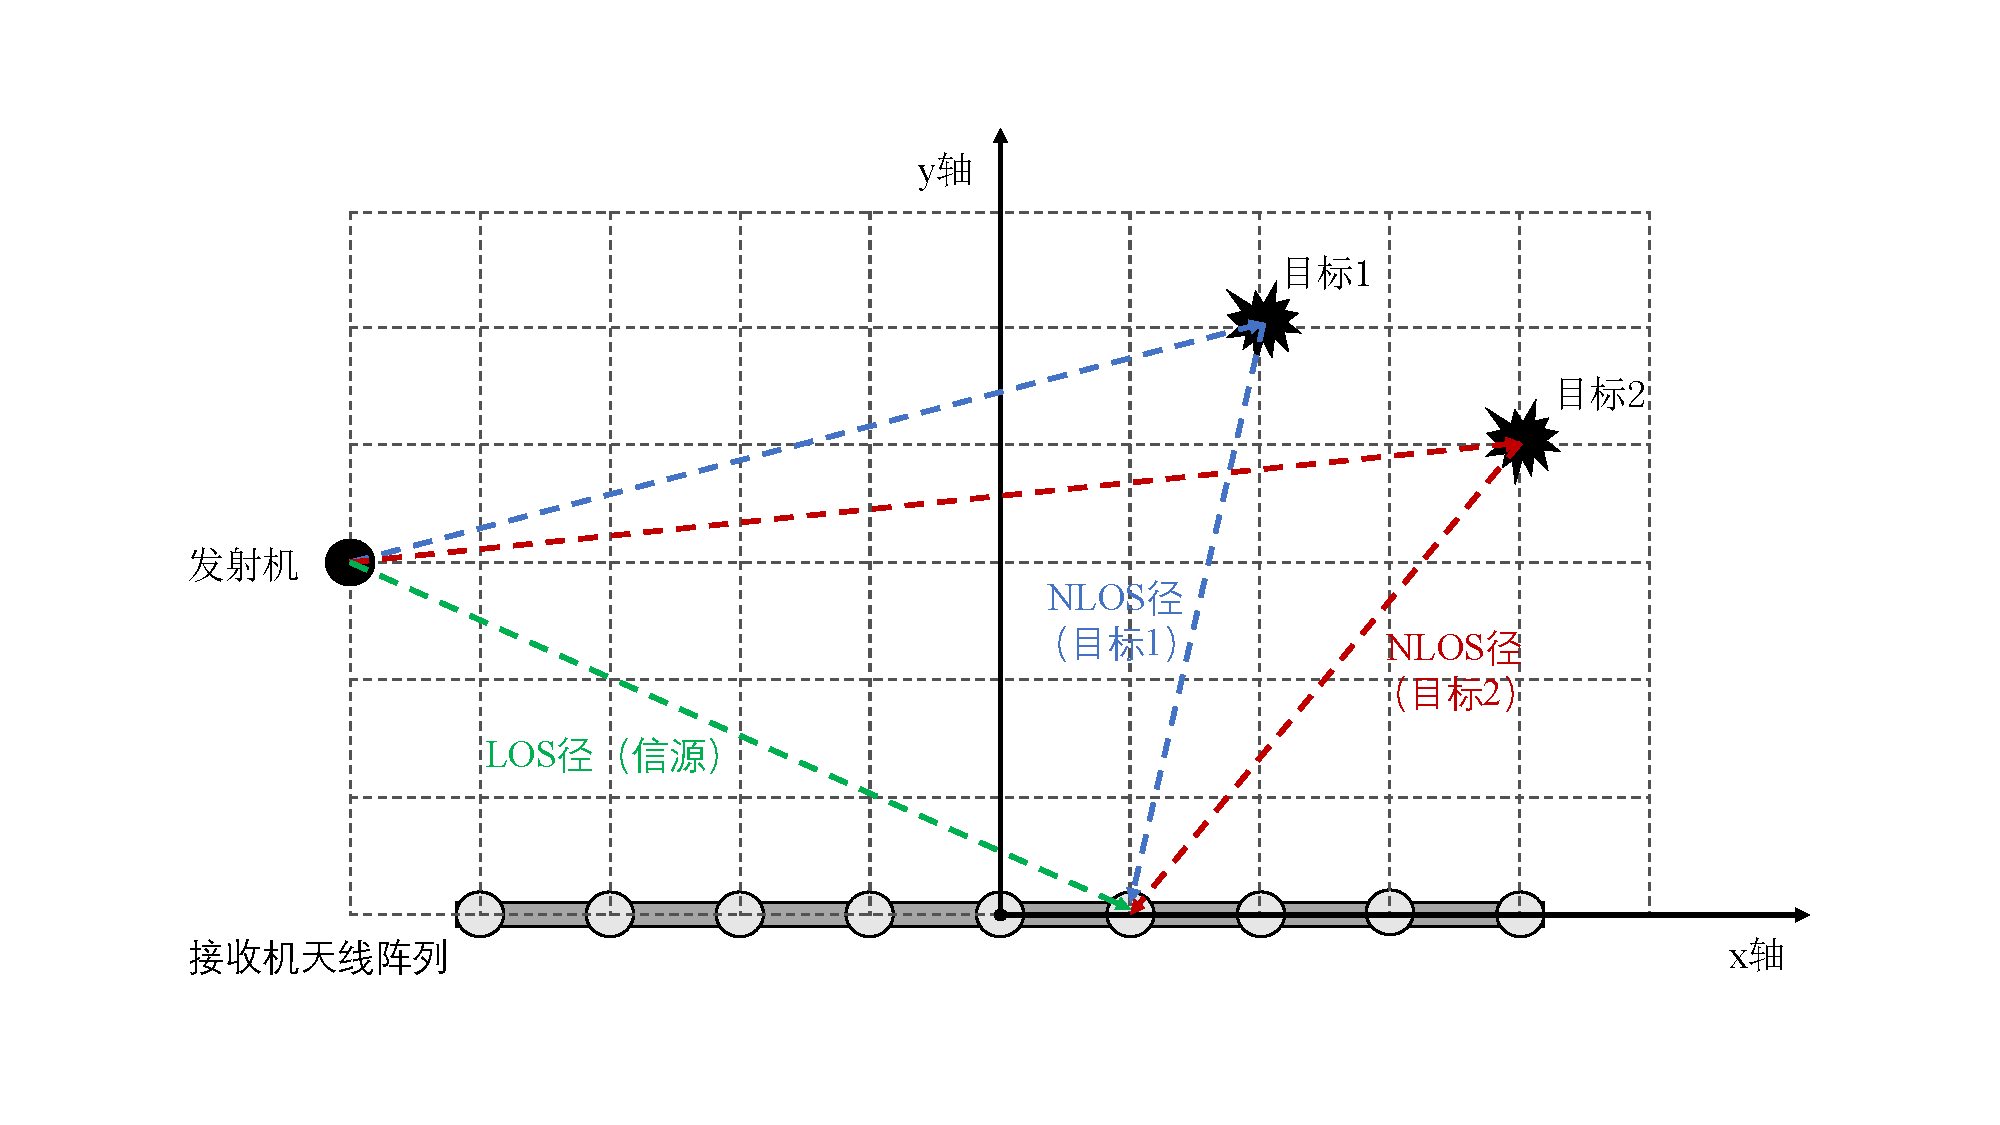
\includegraphics[width=\textwidth]{figures/system_model.pdf}
  \caption{系统模型}
  \label{系统模型}
\end{figure}
(\textbf{系统模型})图~\ref{系统模型}展示了本文所考虑的系统模型。为了方便叙述,这里先讨论的是单个发射机,单个接收机阵
列,两个目标的情形。我们将环境中的两个目标分别表示为:$\text{target}_1$ 和 $\text{target}_2$,设接收机阵列共有$N$个
阵元,并放置于如图的x轴之上。对于整个接收机天线阵列,对接收信号处理所得的CSI为$\boldsymbol{y}=[y_1,\cdots,y_n]^T$,其中第$n$个
阵元所接收的CSI可以表示为发射机对应的一条直射径(LOS: Line Of Sight)与目标对应的两条非直射径
(NLOS: Non Line Of Sight)的叠加\cite{ma2019wifi}:
\begin{align}
  y_n = \underbrace{\alpha_0(n)e^{-j2\pi\frac{d_0(n)}{\lambda}}}_{\text{LOS径}} + \underbrace{\alpha _1(n)e^{ - j2\pi \frac{D_1 + d_1(n)}{\lambda }} + \alpha _2(n)e^{ - j2\pi \frac{D_2 + d_2(n)}{\lambda }}}_{\text{NLOS 径}}\text{,}
\end{align}
其中,$\alpha_0$,$\alpha_1$与$\alpha_2$为幅度衰减因子。$D_1$和 $D_2$分别为发射机到$\text{target}_1$ 和 $\text{target}_2$的距离。$d_0(n)$,$d_1(n)$和$d_2(n)$分别为发射机,$\text{target}_1$和$\text{target}_2$到接收机第$n$个阵元的距离。$\lambda = c/f_c$为Wi-Fi信号的工作波长(在本文后续的仿真与实测中Wi-Fi信号的工作频率$f_c$取$4.2$GHz)。


(\textbf{匹配矩阵构造})将整个感知的平面网格化,针对每一个网格点,根据网格点$(x,y)$到第$n$个接收阵元的距离$(z_n,0)$
的距离$\hat{d}(n)=\sqrt{(x-z_n)^2+y^2}$,可得该网格点与第$n$个接收阵元的相位差为$2\pi\hat{d}(n)/\lambda$,将此设为
网格点$(x,y)$的相位纠正(需要注意的是,我们还可以根据信道衰落与距离的关系,做出相应的幅度补偿,为了便于分析,这里不再讨论)。因此,对于每一个网格点$(x,y)$,我们都有一个匹配向量:
\begin{align}
  \hat{\boldsymbol{y}}=[e^{j2\pi \hat{d}(1)/\lambda} ,\cdots,e^{j2\pi \hat{d}(N)/\lambda}]^T \text{,} \hat{d}(n)=\sqrt{(x-z_n)^2+y^2} \text{。}
  \label{matched array}
\end{align}


(\textbf{匹配滤波})对所有的网格点,将接收的阵列信号$\boldsymbol{y}$与其对应的$\hat{\boldsymbol{y}}$进行匹配,我们可以得到匹配结果:
\begin{align}
  & y_\text{match}  = \boldsymbol{y}^T\hat{\boldsymbol{y}} = \begin{bmatrix}
    \alpha_0(1)e^{-j2\pi\frac{d_0(1)}{\lambda}}+\alpha_1(1)e^{-j2\pi\frac{D_1+d_1(1)}{\lambda}}+\alpha_2(1)e^{-j2\pi\frac{D_2+d_2(1)}{\lambda}} \\
    \vdots \\
    \alpha_0(n)e^{-j2\pi\frac{d_0(n)}{\lambda}}+\alpha_1(n)e^{-j2\pi\frac{D_1+d_1(n)}{\lambda}}+\alpha_2(n)e^{-j2\pi\frac{D_2+d_2(n)}{\lambda}}
  \end{bmatrix}^T
  \begin{bmatrix}
    e^{j2\pi \hat{d}(1)/\lambda} \\
    \vdots \\
    e^{j2\pi \hat{d}(N)/\lambda}  
  \end{bmatrix} \nonumber \\
  & = \sum\limits_{n=1}^N \left(\alpha_0(n)e^{-j2\pi\frac{d_0(n)-\hat{d}(n)}{\lambda}}+\alpha_1(n)e^{-j2\pi\frac{D_1+d_1(n)-\hat{d}(n)}{\lambda}}+\alpha_2(n)e^{-j2\pi\frac{D_2+d_2(n)-\hat{d}(n)}{\lambda}}\right)\text{,}
\end{align}
为了便于分析,我们忽略幅度的影响(假设幅度补偿完美)。在此遍历过程中,有关系式:
\begin{align} 
  & |y_\text{match}| = \left|\sum\limits_{n=1}^N \left(e^{-j2\pi\frac{d_0(n)-\hat{d}(n)}{\lambda}}+e^{-j2\pi\frac{D_1+d_1(n)-\hat{d}(n)}{\lambda}}+e^{-j2\pi\frac{D_2+d_2(n)-\hat{d}(n)}{\lambda}}\right)\right| \nonumber
  \\ 
  & = \left| N + \sum\limits_{n=1}^N \left(e^{-j2\pi\frac{D_1+d_1(n)-\hat{d}(n)}{\lambda}}+e^{-j2\pi\frac{D_2+d_2(n)-\hat{d}(n)}{\lambda}}\right) \right| \text{ 如果}\hat{d}(n)=d_0(n)\text{,信源出现峰值} \nonumber \\
  & = \left| Ne^{-j2\pi\frac{D_1}{\lambda}} +  \sum\limits_{n=1}^N \left(e^{-j2\pi\frac{d_0(n)-\hat{d}(n)}{\lambda}}+e^{-j2\pi\frac{D_2+d_2(n)-\hat{d}(n)}{\lambda}}\right) \right| \text{ 如果}\hat{d}(n)=d_1(n)\text{,目标1出现峰值} \nonumber \\
  & = \left| Ne^{-j2\pi\frac{D_2}{\lambda}} +  \sum\limits_{n=1}^N \left(e^{-j2\pi\frac{d_0(n)-\hat{d}(n)}{\lambda}}+e^{-j2\pi\frac{D_1+d_1(n)-\hat{d}(n)}{\lambda}}\right) \right| \text{ 如果}\hat{d}(n)=d_2(n)\text{,目标2出现峰值} \nonumber \\
  & \approx N \text{,}
\end{align}
从上述公式可以看出,在网格点遍历的过程中,对应信源,目标的网格点会出现峰值,关于这一现象,我们会在小节2.3给出详细的仿真。
\subsection{理想仿真成像}
本小节,我们给出更加详细的理想仿真成像模型,将上一小节的情形扩展到了环境之中存在1个发射机和$L$个目标($\text{target}_1,\cdots,\text{target}_L$)的情况,我们有:
\begin{itemize}
  \item 天线信号的接收信号$\boldsymbol{y}=[y_1,\cdots,y_n]^T$可以表示为发射机对应的一条直射径和$L$条目标对应的非直射径的叠加:
  \begin{align}
    y_n &= \underbrace{\alpha_0(n)e^{-j2\pi\frac{d_0(n)}{\lambda}}}_{\text{LOS径}} + \underbrace{\alpha _1(n)e^{ - j2\pi \frac{D_1 + d_1(n)}{\lambda }} + \cdots + \alpha _L(n)e^{ - j2\pi \frac{D_L + d_L(n)}{\lambda }}}_{L\text{条NLOS 径}} \nonumber \\
    &= \sum_{l=0}^L \alpha_l e^{-j 2\pi \frac{D_l + d_l(n)}{\lambda}} \text{,}
  \end{align}
  这里$\{\alpha_l\}_{l\in \mathcal{L}}$,$\{D_l\}_{l\in \mathcal{L}}$,$\{d_l\}_{l \in \mathcal{L}}$分别指第$l$条多径的幅度衰减因子的集合,发射机到$\text{target}_l$的距离的集合($D_0 = 0$),$\text{target}_l$到接收机的距离的集合。$\mathcal{L}=\{0,1,\cdots,L\}$为多径的下标集合($l=0$指LOS径,对应信源)。
  \item 匹配矩阵$\hat{\boldsymbol{y}}$仍然保持公式~\eqref{matched array}的形式。
  \begin{itemize}
    \item 需要注意的是,这里的匹配矩阵只需要计算一次。
  \end{itemize}
  \item 同样忽略幅度影响,可得匹配的结果:
  \begin{align}
    &|y_{\text{match}}| = |\boldsymbol{y}^T\hat{\boldsymbol{y}}| = \left| \sum\limits_{n=1}^N \sum\limits_{l=0}^{L}e^{-j2\pi\frac{D_l+d_l(n)-\hat{d}(n)}{\lambda}} \right| \nonumber \\
    & = \left| N + \sum\limits_{n=1}^N\sum_{l \in \mathcal{L}/\{0\}}e^{-j2\pi\frac{D_l+d_l(n)-\hat{d}(n)}{\lambda}}  \right| \text{ 如果}\hat{d}(n)=d_0(n)\text{,信源出现峰值} \nonumber \\ 
    & = \cdots \nonumber \\
    & = \left| Ne^{-j2\pi D_i\lambda} + \sum\limits_{n=1}^N\sum_{l \in \mathcal{L}/\{i\}}e^{-j2\pi\frac{D_l+d_l(n)-\hat{d}(n)}{\lambda}}  \right| \text{ 如果}\hat{d}(n)=d_i(n)\text{,目标}i\text{出现峰值} \nonumber \\
    & = \cdots \nonumber \\
    & = \left| Ne^{-j2\pi D_L\lambda} + \sum\limits_{n=1}^N\sum_{l \in \mathcal{L}/\{L\}}e^{-j2\pi\frac{D_L+d_L(n)-\hat{d}(n)}{\lambda}}  \right| \text{ 如果}\hat{d}(n)=d_L(n)\text{,目标}L\text{出现峰值} \nonumber \\
    & \approx N \text{。}
  \end{align}
  \item 为了使成像峰值更加明显,我们后续还对成像结果进行了归一化以及加窗(汉明窗)处理。
\end{itemize}
\subsection{理想成像仿真结果}
本小节展示了理想状态下的成像仿真,仿真设置见表~\ref{理想成像仿真设置}:
\begin{table}[htb]
  % h-here,t-top,b-bottom,优先级依次下降
      \begin{center}
      % 居中
          \caption{理想成像仿真设置}\label{理想成像仿真设置}
          \begin{tabular}{lc} % 三线表不能有竖线,l-left,c-center,r-right
              \toprule
              %三线表-top 线
              参数 & 值 \\
              \midrule
              %三线表-middle 线
              是否考虑对信源(发射机)成像 & 否,仿真多径没有设置LOS径\\
              是否考虑CSI频偏的影响 & 否,该小节测试理想成像的结果\\
              成像目标数量    & 3\\
              成像目标的位置  & $(1\text{米},1\text{米})$,$(2\text{米},1.5\text{米})$,$(3\text{米},2\text{米})$ \\
              工作频点        & $4.2$GHz\\
              工作带宽      & 20MHz \\
              子载波数目      & 256\\
              发射机位置           & $(2\text{米},0\text{米})$\\
              接收机天线阵元数$N$      & $32$,$64$,$128$\\
              接收机天线阵元间隔    & 半波长(约$3.57$厘米)\\
              接收机位置           & 类似图~\ref{系统模型},阵列中心位于原点\\
              \bottomrule
              %三线表-底线
          \end{tabular}
      \end{center}
\end{table}

需要注意的是:
\begin{itemize}
  \item 仿真考虑类似图~\ref{系统模型}中的单接收机阵列对三个目标进行成像(最初没有考虑对信源成像,但其实信源的成像与目标的成像是等效的);
  \item 仿真其实只利用了一个子载波上的信号进行成像,如何利用多载波上的CSI联合成像以提升成像性能是一个可能的拓展方向。 
  \item 本小节的仿真并没有考虑CSI频偏的影响,旨在得到一个``完美的''理想成像结果,作为后续考虑频偏成像的上界作为对比。
\end{itemize}

理想成像仿真结果如图~\ref{理想成像仿真结果}所示:

\begin{figure}[htb]
  \centering
  \begin{subfigure}[t]{.45\linewidth}
      \centering
      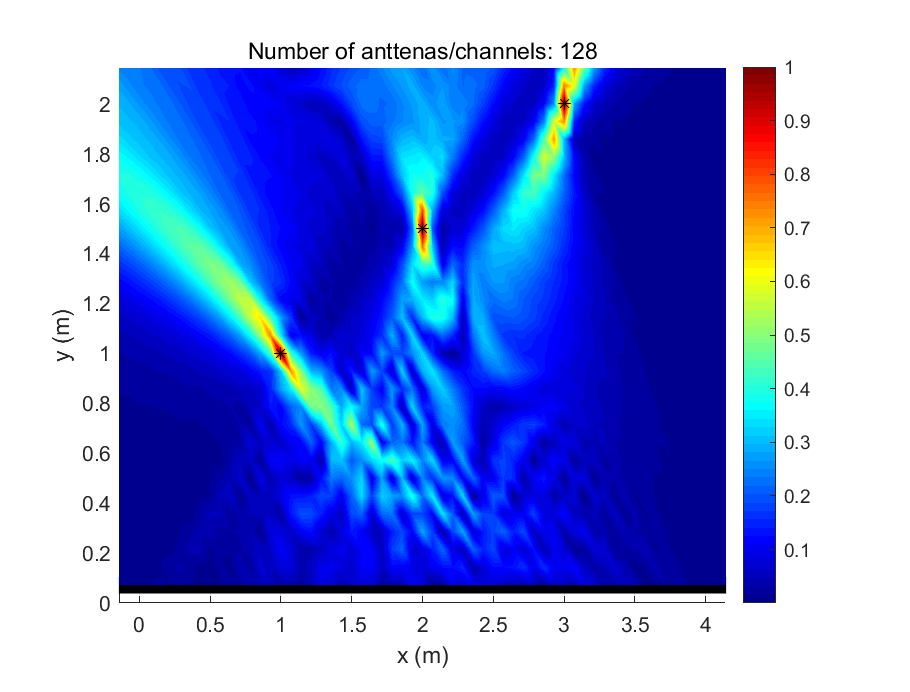
\includegraphics[width=1\textwidth]{figures/expected/128.eps}
      \caption{接收机天线阵元数$N=128$}
  \end{subfigure}
  \begin{subfigure}[t]{.45\linewidth}
      \centering
      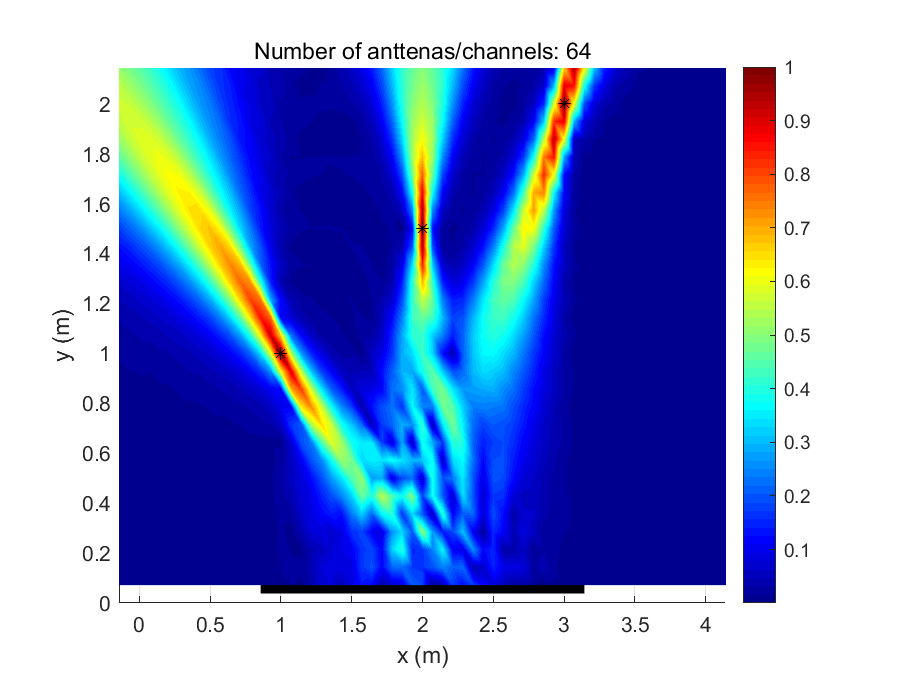
\includegraphics[width=1\textwidth]{figures/expected/64.eps}
      \caption{接收机天线阵元数$N=64$}
  \end{subfigure}
  \\
  \begin{subfigure}[t]{.45\linewidth}
    \centering
    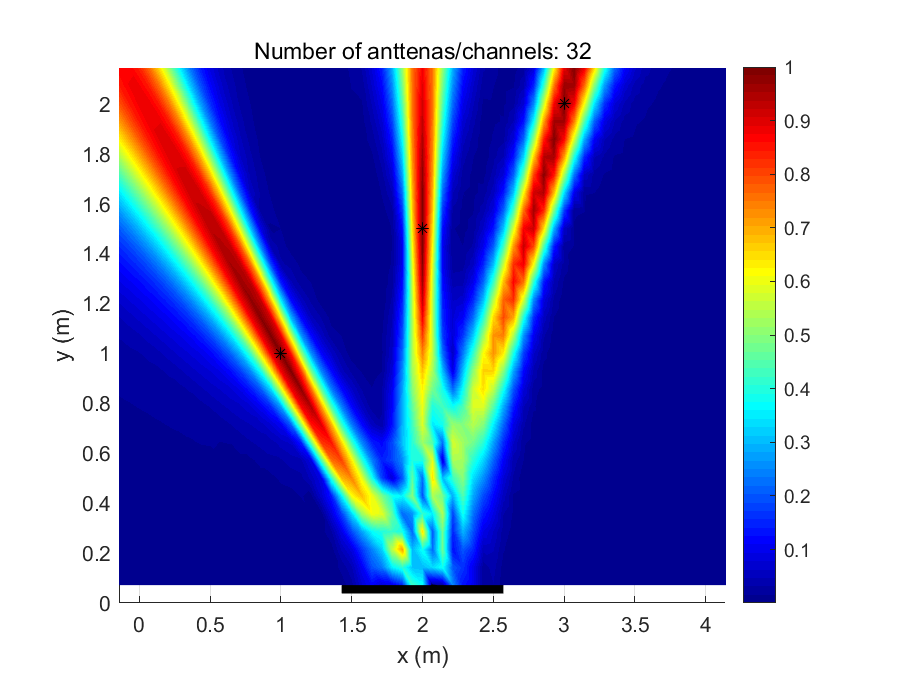
\includegraphics[width=1\textwidth]{figures/expected/32.eps}
    \caption{接收机天线阵元数$N=32$}
\end{subfigure}
  \caption{理想成像仿真结果}\label{理想成像仿真结果}
\end{figure}
仿真结果表明,理想的仿真成像可以良好的对目标进行检测,定位,和成像。 
  \section{考虑频偏消除的成像仿真}
\subsection{CSI频偏模型}
在实际的通信系统中,测量得到的CSI会受到多径效应,收发机的不同步处理,以及软/硬件上存在的客观误差等因素的
影响,导致受到频偏的影响。最主要的频偏影响因素有:采样频率偏移(SFO: Sampling Frequency Offset),以及
包检测误差(PDD: Packet Detection Delay)以及载波频率偏移(CFO: Carrier Frequency Offset)等\cite{ma2019wifi}\cite{Precise_PDP_WiFi}。
受以上因素影响的接收信号(CSI)$\tilde{\boldsymbol{y}}$将满足如下表达式\cite{zhang2022practical}:
\begin{align}
  \tilde{\boldsymbol{y}} &= \boldsymbol{y}e^{-j\theta_{\text{offset}}(t)} \nonumber 
  \\ &= \boldsymbol{y}e^{-j \left\{2\pi f[\theta_{\text{SFO}}(t)+\theta_{\text{PDD}}(t)]+2\pi \theta_{\text{CFO}}(t)\right\}}
  \text{。}
\end{align}
本文考虑的两种频偏情形:
\begin{enumerate}
  \item (类似SAR的情形)这种频偏的情形与我们后续实测时利用轨道移动模拟天线阵列一致,信号到达阵列上每一个点的频偏不一致。
  \begin{align}
    & \text{(情形一)}\quad \tilde{\boldsymbol{y}} = \boldsymbol{y}e^{-j\theta_{\text{offset}}} \nonumber \\
    &= \boldsymbol{y} \odot \left[e^{-j\left\{-j2\pi f[\theta_{\text{SFO},1}+\theta_{\text{PDD},1}]+2\pi \theta_{\text{CFO},1}\right\}},\cdots,e^{-j\left\{-j2\pi f[\theta_{\text{SFO},N}+\theta_{\text{PDD},N}]+2\pi \theta_{\text{CFO},N}\right\}}\right]^T
    \text{。}
    \label{情形一}
  \end{align}
  这里$\odot$指的是矩阵的点乘。
  \item (类似图~\ref{系统模型}一个巨大的接收阵列的情形)当然,我们考虑信号同时到达我们的天线阵列(考虑某一时刻的CSI),则有:
  \begin{align}
    \text{(情形二)}\quad
    \tilde{\boldsymbol{y}} = \boldsymbol{y}e^{-j\{2\pi f[\theta_{\text{SFO}}+\theta_{\text{PDD}}]+2\pi\theta_{\text{CFO}}\}}
    \text{。}
    \label{情形二}
  \end{align}
\end{enumerate}


如果不消除频偏,由于我们主要根据相位匹配滤波,会导致成像的某些径的峰值不够明显,各个目标成像峰值差距过大,成像模糊以及成像模糊等问题
(具体的仿真结果将与本文频偏消除后的结果,共同于小节~3.4介绍)。
\subsection{CSI频偏消除的方法}
目前主流的CSI频偏消除的方式主要有两种类型\cite{ma2019wifi}:
\begin{enumerate}
  \item 基于相位相位``相减''的方式\cite{wu2021wifi}。
  \begin{itemize}
    \item 两路CSI信号共轭相乘。
    \begin{align}
      \tilde{\boldsymbol{y}_1}\times\tilde{\boldsymbol{y}_2}^H = (\boldsymbol{y}_1e^{-j\theta_{\text{offset}}})\times(\boldsymbol{y}_2e^{-j\theta_{\text{offset}}})^H
      \text{,}
    \end{align}
    \item 两路CSI信号相除。
    \begin{align}
      \tilde{\boldsymbol{y}_1}/\tilde{\boldsymbol{y}_2} = (\boldsymbol{y}_1e^{-j\theta_{\text{offset}}})/(\boldsymbol{y}_2e^{-j\theta_{\text{offset}}})
      \text{。}
    \end{align}
  \end{itemize}
  \item 基于线性拟合的方法。
  \begin{itemize}
    \item 文章SignFi\cite{SignFi}提出了一种沿着CSI子载波与天线维度最小化拟合误差的方法:
    \begin{align}
      \rho^*, \beta^* = \arg \limits_{\rho,\beta} \min \sum_{r,f}(\Theta_{r,f} + 2\pi f \rho + \beta)^2
      \text{,}
    \end{align}
    这里,$\Theta_{r,f}$是测量得到的CSI相位,$\rho$与$\beta$是拟合的参数。如果拟合完美,我们可以近似的得到:
    $\rho^* = \theta_{\text{SFO}} + \theta_{\text{PDD}}$以及$\beta^*/(2\pi) = \theta_{\text{CFO}}$。
  \end{itemize}
\end{enumerate}


为了简单考虑,本文后续主要考虑了基于两路CSI信号共轭相乘的方式消除频偏。仿真结果在小节~3.4介绍。
\subsection{结合CSI共轭相乘和PARAFAC算法的频偏消除成像}
直接利用两路CSI信号共轭相乘,然后对多径信号直接成像的操作并不完美,主要体现在:
\begin{enumerate}
  \item 对于接收两路CSI的天线,要求一个较大的天线间距。
  \item 对于某些目标,峰值不够明显,甚至无法被检测到。
\end{enumerate}

为了克服以上问题,将多径信号分离出来,再对每一条多径分别消除频偏并成像是一个可行的方案。
本小节基于平行因子分析(PARAFAC,Parallel Factor)中的TPF (Trilinear Parallel Factor)
技术中的复平行因子分析算法(COMFAC, Complex parallel Factor Analysis)\cite{bro1999fast},估计接收信号
的每一条径的CSI\cite{TPF}。之后对每一条径的CSI分别做共轭相乘操作以消除频偏,并分别成像。


目前所采用的TPF估计原理如下:
\begin{itemize}
  \item 假设在某一时刻,有两路(带有频偏的)接收信号$\widetilde{\boldsymbol{y}_1},\widetilde{\boldsymbol{y}_2} \in \mathbb{C}^{F\times N}$,这里$F$为子载波数目,
  $N$为接收天线的数目。
  \item 将以二维的CSI转化为三维矩阵的形式$\widetilde{\boldsymbol{Y}}_1,\widetilde{\boldsymbol{Y}}_2$。转化为三维矩阵的方式很多,这里选择使用切片滑窗的方式。
  \begin{itemize}
    \item 设定一个切片间隔$P$,通过不断截取源CSI的$P$子载波间隔,将其存为CSI的一个新维度,可以得到重构的三维的CSI满足:
    $\widetilde{\boldsymbol{Y}}_1,\widetilde{\boldsymbol{Y}}_2 \in \mathbb{C}^{P\times N \times (F-P+1)}$
  \end{itemize}
  \item 对这两个三维的CSI分别运行COMFAC算法(需要指定目标数量$L$)得到其对应的平行因子$\{\boldsymbol{A}_1,\boldsymbol{B}_1,\boldsymbol{C}_1\}$和$\{\boldsymbol{A}_2,\boldsymbol{B}_2,\boldsymbol{C}_2\}$。
  其中,$\boldsymbol{A}_1,\boldsymbol{A}_2\in \mathbb{C}^{P\times L}$,$\boldsymbol{B}_1,\boldsymbol{B}_2\in \mathbb{C}^{N \times L}$,$\boldsymbol{C}_1,\boldsymbol{C}_2\in \mathbb{C}^{(F-P+1)\times L}$。
  \item 我们有:
  \begin{align}
    &{\widetilde {\boldsymbol{Y}}_1}(i,j,k) = \sum\limits_{l = 1}^L {{{\widetilde {\boldsymbol{Y}}}^l}_1(i,j,k)}  = \sum\limits_{l = 1}^L {{{\boldsymbol{A}}_1}(i,l){{\boldsymbol{B}}_1}(j,l){{\boldsymbol{C}}_1}(k,l) + {{\boldsymbol{E}}_1}(i,j,k)} \nonumber \\
    &{\widetilde {\boldsymbol{Y}}_2}(i,j,k) = \sum\limits_{l = 1}^L {{{\widetilde {\boldsymbol{Y}}}^l}_2(i,j,k)}  = \sum\limits_{l = 1}^L {{{\boldsymbol{A}}_2}(i,l){{\boldsymbol{B}}_2}(j,l){{\boldsymbol{C}}_2}(k,l) + {{\boldsymbol{E}}_2}(i,j,k)} \nonumber \\
    &l = 1, \ldots ,L;\quad \,i = 1, \ldots ,P;j = 1, \ldots ,N;\quad k = 1, \ldots ,F - P + 1
    \label{TPF_decomp}
  \end{align}
  其中,$\boldsymbol{E}_1(i,j,k)$和$\boldsymbol{E}_2(i,j,k)$为三线性模型的误差。
  $\widetilde{\boldsymbol{Y}}^l_1(i,j,k)$和$\widetilde{\boldsymbol{Y}}^l_1(i,j,k)$为COMFAC算法估计得到的两路CSI第$l$条径的三维形式。
  \item 将三维形式的多径CSI$\left\{\tilde{\boldsymbol{Y}}^l_1\right\}_{l\in\mathcal{L}}$和$\left\{\tilde{\boldsymbol{Y}}^l_2\right\}_{l\in\mathcal{L}}$ 
  转化为二维形式的多径CSI:$\left\{\tilde{\boldsymbol{y}}^l_1\right\}_{l\in\mathcal{L}}$和$\left\{\tilde{\boldsymbol{y}}^l_2\right\}_{l\in\mathcal{L}}$。
  对两路CSI分别共轭相乘消除频偏,并匹配成像即可。
\end{itemize}
需要注意的是:
\begin{enumerate}
  \item 公式~\eqref{TPF_decomp}所表示的三线性因子分解具有唯一性,这一点由Kruskal, Joseph B于1989年最先证明\cite{kruskal1989rank}。
  \item COMFAC算法是求解平行因子分解的其中一种快速算法,典型的方法还有三线性交替最小二乘回归(TALS: Trilinear Alternating Least Square Regression)算法等\cite{TPF}。
  \item 本文不详细介绍COMFAC算法的具体实现过程,后续仿真中直接使用了明尼苏达大学Nikos D. Sidiropoulos团队关于COMFAC算法的开源代码\cite{COMFAC_matlab}。
\end{enumerate}

\subsection{考虑频偏消除的成像仿真结果对比}
本小节给出考虑频偏影响下,共轭相乘消除频偏,结合PARFAC算法与共轭相乘消除频偏的成像仿真及对比,仿真参数如表~\ref{共轭相乘成像和结合PARAFAC与共轭相乘成像}所示
(需要注意的是这里添加了一个新的参数$\Delta_d$代表两路接收天线的位置差)。
\begin{table}[htb]
  % h-here,t-top,b-bottom,优先级依次下降
      \begin{center}
      % 居中
          \caption{共轭相乘成像和结合PARAFAC与共轭相乘成像仿真设置}\label{共轭相乘成像和结合PARAFAC与共轭相乘成像}
          \begin{tabular}{lc} % 三线表不能有竖线,l-left,c-center,r-right
              \toprule
              %三线表-top 线
              参数 & 值 \\
              \midrule
              %三线表-middle 线
              是否考虑对信源(发射机)成像 & 否,仿真多径没有设置LOS径\\
              是否考虑CSI频偏的影响 & 是\\
              考虑频偏的情形  & 服从公式~\eqref{情形二}\\
              采样频率偏移(SFO)   &   $\theta_{\text{sfo}}\sim N(0,100)$ Hz\\
              包检测误差(PDP)     &   $\theta_{\text{pdd}}\sim N(0,100)$ Hz\\
              载波频率偏移(CFO)   &   $\theta_{\text{cfo}}\sim N(0,1000)$ Hz\\
              成像目标数量    & 3\\
              成像目标的位置  & $(1\text{米},1\text{米})$,$(2\text{米},1.5\text{米})$,$(3\text{米},2\text{米})$ \\
              工作频点        & $4.2$GHz\\
              工作带宽      & 20MHz \\
              子载波数目      & 256\\
              发射机位置           & $(0\text{米},0\text{米})$\\
              接收机天线阵元数$N$      & $32$,$64$,$128$\\
              接收机天线阵元间隔    & 半波长(约$3.57$厘米)\\
              接收机位置           & 类似图~\ref{系统模型},阵列中心位于原点\\
              两路接收天线的位置差$\Delta_d$ & $10$米,$3$米,$0.5$米\\
              \bottomrule
              %三线表-底线
          \end{tabular}
      \end{center}
\end{table}
\begin{table}[htb]
  % h-here,t-top,b-bottom,优先级依次下降
      \begin{center}
      % 居中
          \caption{不消除频偏、共轭相乘成像、结合PARAFAC与共轭相乘成像对比仿真设置}\label{对比}
          \begin{tabular}{lc} % 三线表不能有竖线,l-left,c-center,r-right
              \toprule
              %三线表-top 线
              参数 & 值 \\
              \midrule
              %三线表-middle 线
              是否考虑对信源(发射机)成像 & 否,仿真多径没有设置LOS径\\
              是否考虑CSI频偏的影响 & 是,既考虑添加频偏又考虑不添加频偏的成像\\
              考虑频偏的情形  & 考虑公式~\eqref{情形一}\eqref{情形二}两种情形\\
              采样频率偏移(SFO)   &   $\theta_{\text{sfo}}\sim N(0,100)$ Hz\\
              包检测误差(PDP)     &   $\theta_{\text{pdd}}\sim N(0,100)$ Hz\\
              载波频率偏移(CFO)   &   $\theta_{\text{cfo}}\sim N(0,1000)$ Hz\\
              成像目标数量    & 3\\
              成像目标的位置  & $(1\text{米},1\text{米})$,$(2\text{米},1.5\text{米})$,$(3\text{米},2\text{米})$ \\
              工作频点        & $4.2$GHz\\
              工作带宽      & 20MHz \\
              子载波数目      & 256\\
              发射机位置           & $(0\text{米},0\text{米})$\\
              接收机天线阵元数$N$      & $32$\\
              接收机天线阵元间隔    & 半波长(约$3.57$厘米)\\
              接收机位置           & 类似图~\ref{系统模型},阵列中心位于原点\\
              两路接收天线的位置差$\Delta_d$ & $3$米\\
              \bottomrule
              %三线表-底线
          \end{tabular}
      \end{center}
\end{table}

\clearpage
图~\ref{共轭相乘消除频偏成像结果}展示了共轭相乘消除频偏成像仿真结果:
\begin{figure}[H]
  \centering
  \begin{subfigure}[t]{.45\linewidth}
      \centering
      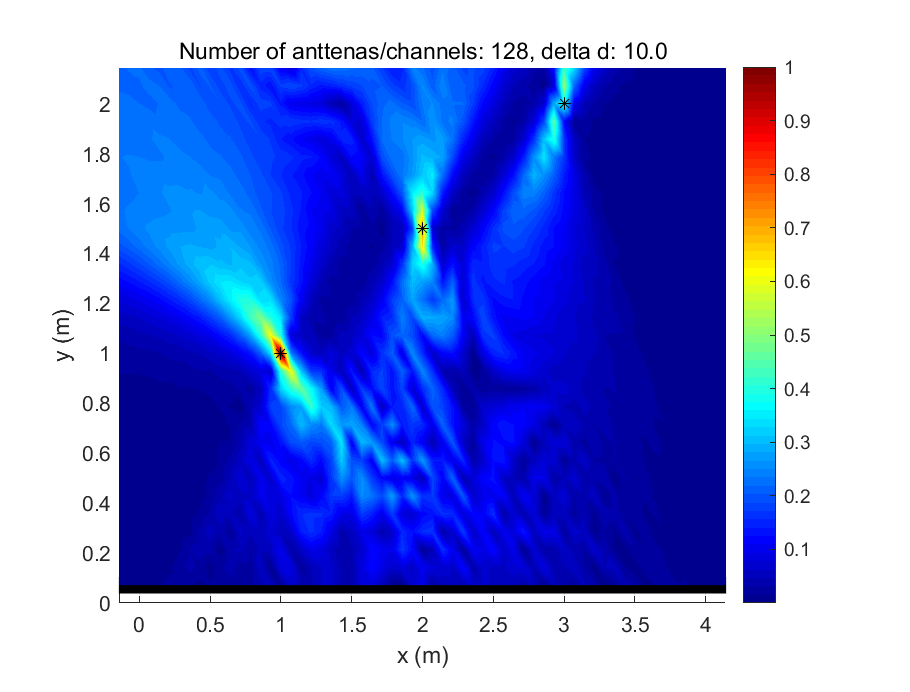
\includegraphics[width=1\textwidth]{figures/cm/N128d10.eps}
      \caption{接收机天线阵元数$N=128$,$\Delta_d = 10\text{m}$}
  \end{subfigure}
  \begin{subfigure}[t]{.45\linewidth}
      \centering
      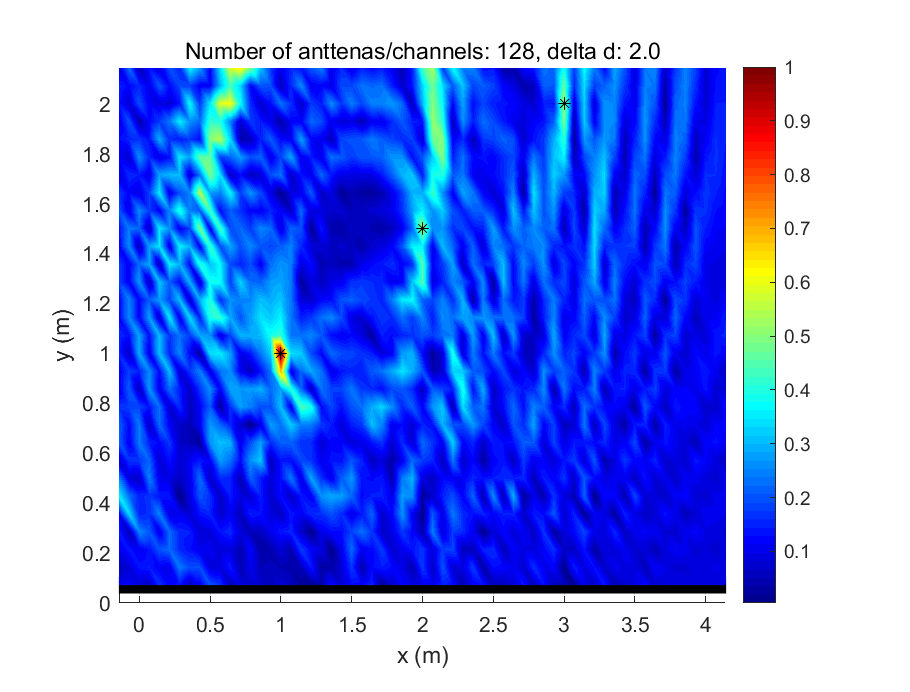
\includegraphics[width=1\textwidth]{figures/cm/N128d2.eps}
      \caption{接收机天线阵元数$N=128$,$\Delta_d = 2\text{m}$}
  \end{subfigure}
  \\
  \begin{subfigure}[t]{.45\linewidth}
    \centering
    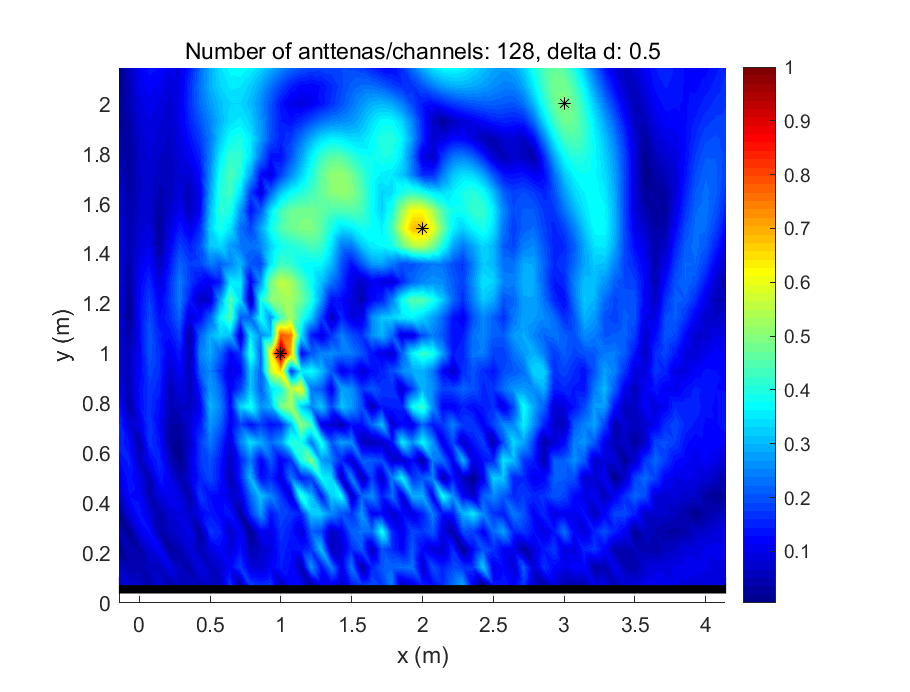
\includegraphics[width=1\textwidth]{figures/cm/N128d0.5.eps}
    \caption{接收机天线阵元数$N=128$,$\Delta_d = 0.5\text{m}$}
  \end{subfigure}
  \begin{subfigure}[t]{.45\linewidth}
    \centering
    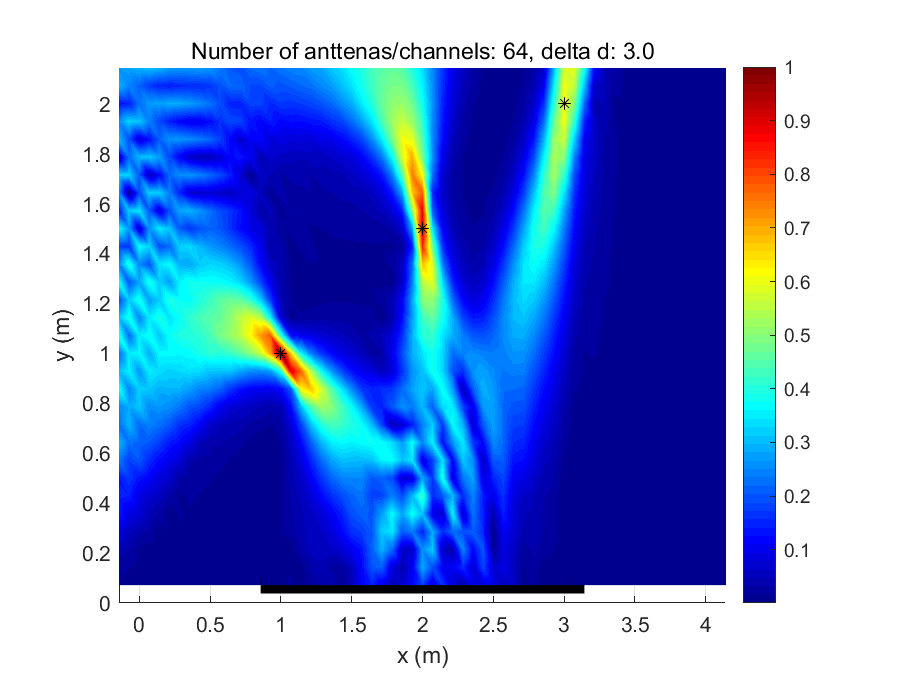
\includegraphics[width=1\textwidth]{figures/cm/N64d3.eps}
    \caption{接收机天线阵元数$N=64$,$\Delta_d = 3\text{m}$}
  \end{subfigure}
  \\
  \begin{subfigure}[t]{.45\linewidth}
    \centering
    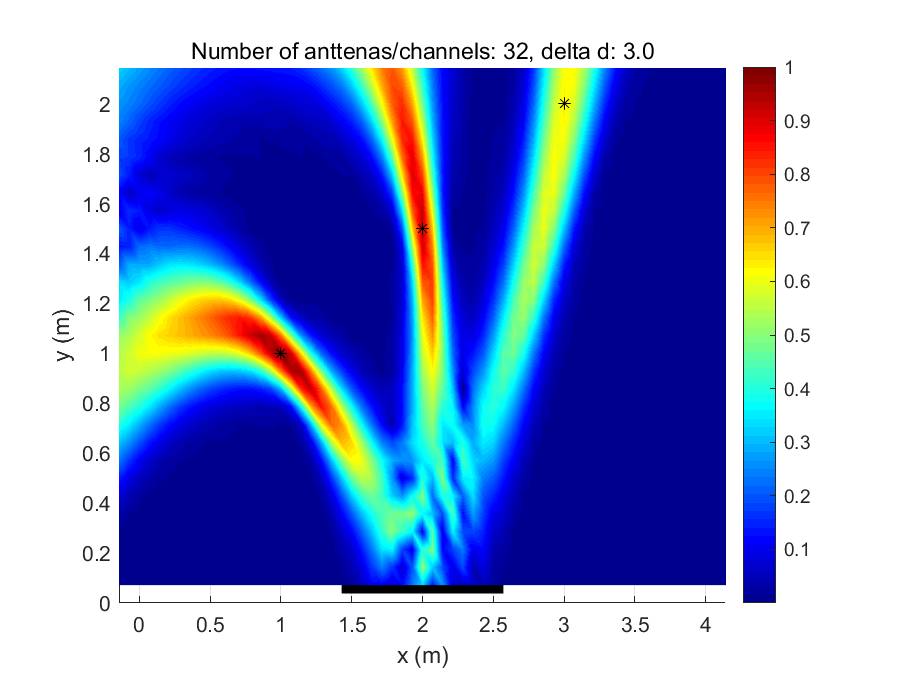
\includegraphics[width=1\textwidth]{figures/cm/N32d3.eps}
    \caption{接收机天线阵元数$N=32$,$\Delta_d = 3\text{m}$}
  \end{subfigure}
  \caption{共轭相乘消除频偏成像结果}\label{共轭相乘消除频偏成像结果}
\end{figure}


图~\ref{结合PARAFAC算法与共轭相乘消除频偏成像仿真结果}展示了结合PARAFAC算法与共轭相乘消除频偏成像仿真结果:
\begin{figure}[H]
  \centering
  \begin{subfigure}[t]{.45\linewidth}
      \centering
      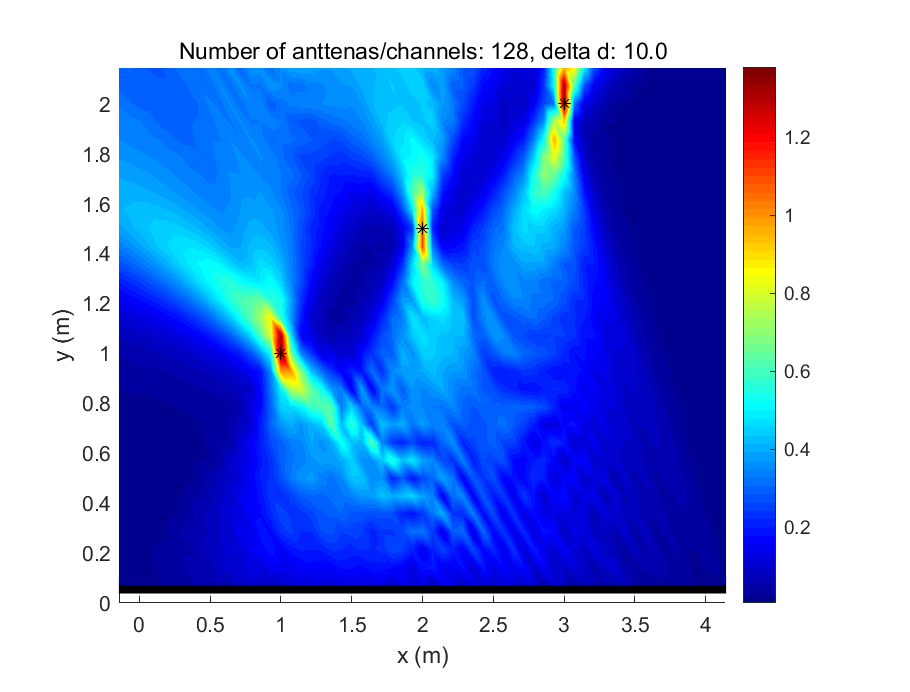
\includegraphics[width=1\textwidth]{figures/TPF/N128d10.eps}
      \caption{接收机天线阵元数$N=128$,$\Delta_d = 10\text{m}$}
  \end{subfigure}
  \begin{subfigure}[t]{.45\linewidth}
      \centering
      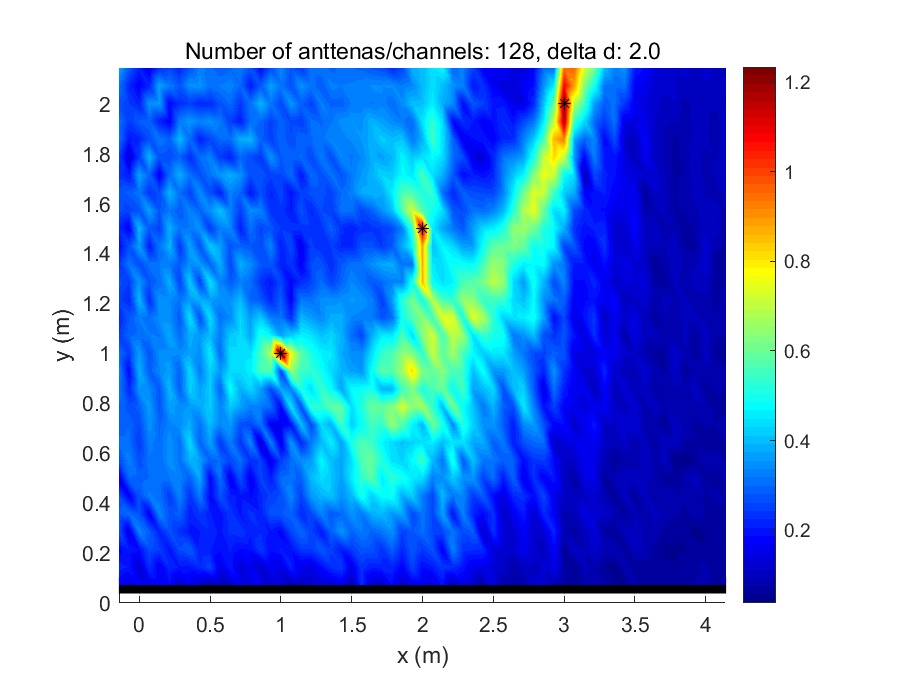
\includegraphics[width=1\textwidth]{figures/TPF/N128d2.eps}
      \caption{接收机天线阵元数$N=128$,$\Delta_d = 2\text{m}$}
  \end{subfigure}
  \\
  \begin{subfigure}[t]{.45\linewidth}
    \centering
    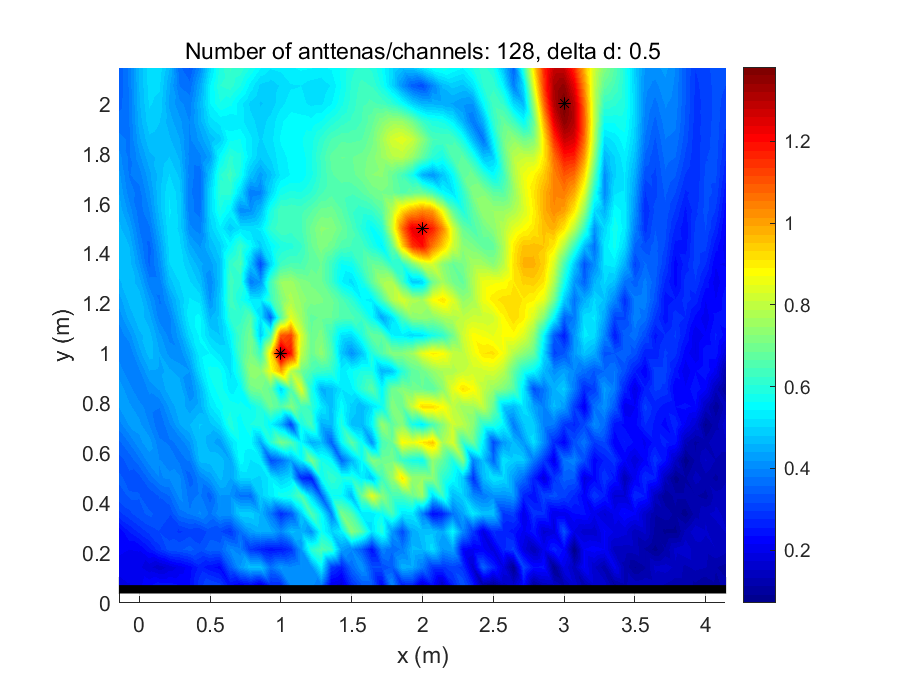
\includegraphics[width=1\textwidth]{figures/TPF/N128d0.5.eps}
    \caption{接收机天线阵元数$N=128$,$\Delta_d = 0.5\text{m}$}
  \end{subfigure}
  \begin{subfigure}[t]{.45\linewidth}
    \centering
    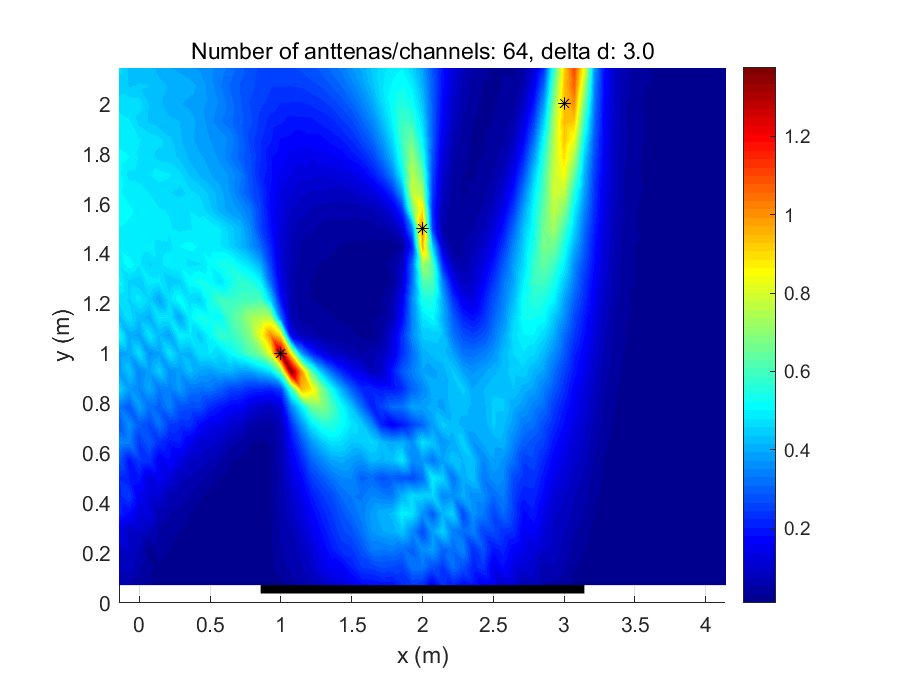
\includegraphics[width=1\textwidth]{figures/TPF/N64d3.eps}
    \caption{接收机天线阵元数$N=64$,$\Delta_d = 3\text{m}$}
  \end{subfigure}
  \\
  \begin{subfigure}[t]{.45\linewidth}
    \centering
    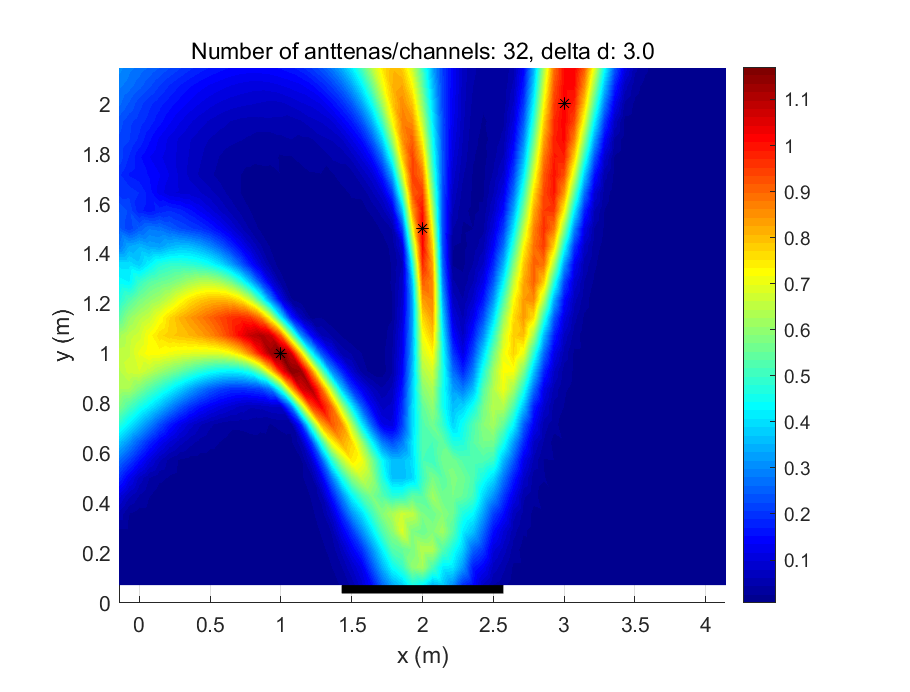
\includegraphics[width=1\textwidth]{figures/TPF/N32d3.eps}
    \caption{接收机天线阵元数$N=32$,$\Delta_d = 3\text{m}$}
  \end{subfigure}
  \caption{结合PARAFAC算法与共轭相乘消除频偏成像仿真结果}\label{结合PARAFAC算法与共轭相乘消除频偏成像仿真结果}
\end{figure}


将图~\ref{共轭相乘消除频偏成像结果}与图~\ref{结合PARAFAC算法与共轭相乘消除频偏成像仿真结果}对比,可以看出
结合PARAFAC的共轭相乘消除频偏的成像具有更加明显的峰值,但是都需要一个大的天线阵列,以及一个较大的两路天线阵列的间隔。


为了更好的展示成像的差别,根据表~\ref{对比},我们在接收天线数量$N=32$的情形下,考虑公式\eqref{情形一},\eqref{情形二}两种频偏模型,
对不消除频偏直接成像,不消除频偏并利用PARAFAC算法增强峰值直接成像,共轭相乘消除频偏成像,结合CSI共轭相乘和PARAFAC算法消除频偏等
四种成像进行了对比,见图~\ref{成像对比图}。可以看出,自发自收与情形二的仿真结果一致,说明如果我们有一个足够长的天线阵列,则不需要频偏消除。
PARAFAC算法可以有效增强峰值,但目前在情形一仍然不能太好的处理频偏。


\begin{figure}[H]
  \centering
  \begin{subfigure}[t]{.3\linewidth}
    \centering
    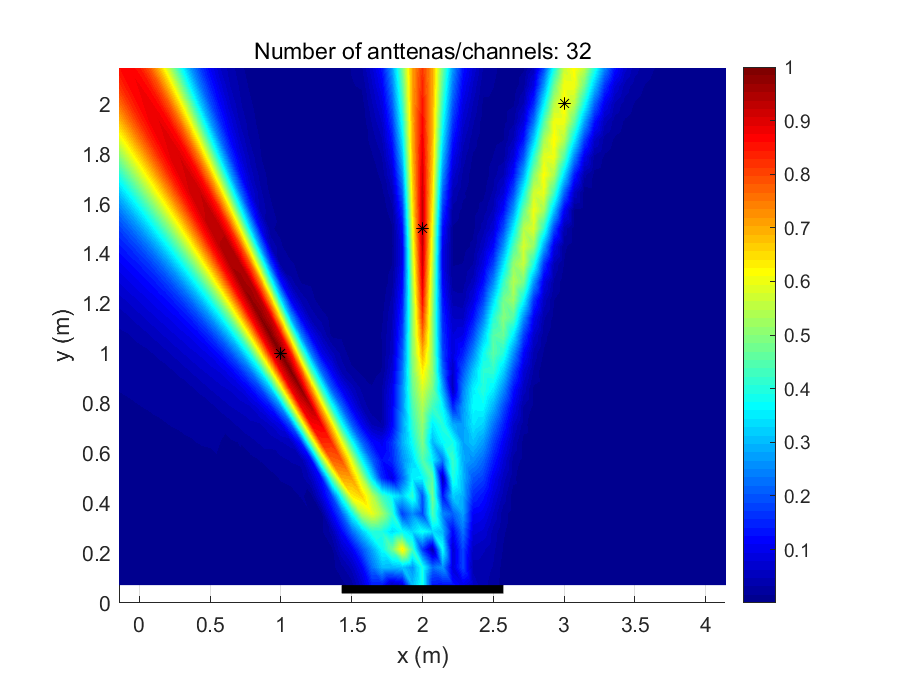
\includegraphics[width=1\textwidth]{figures/compare/CSI_without_freq.eps}
    \caption{未添加频偏~直接成像}
  \end{subfigure}
  \begin{subfigure}[t]{.3\linewidth}
    \centering
    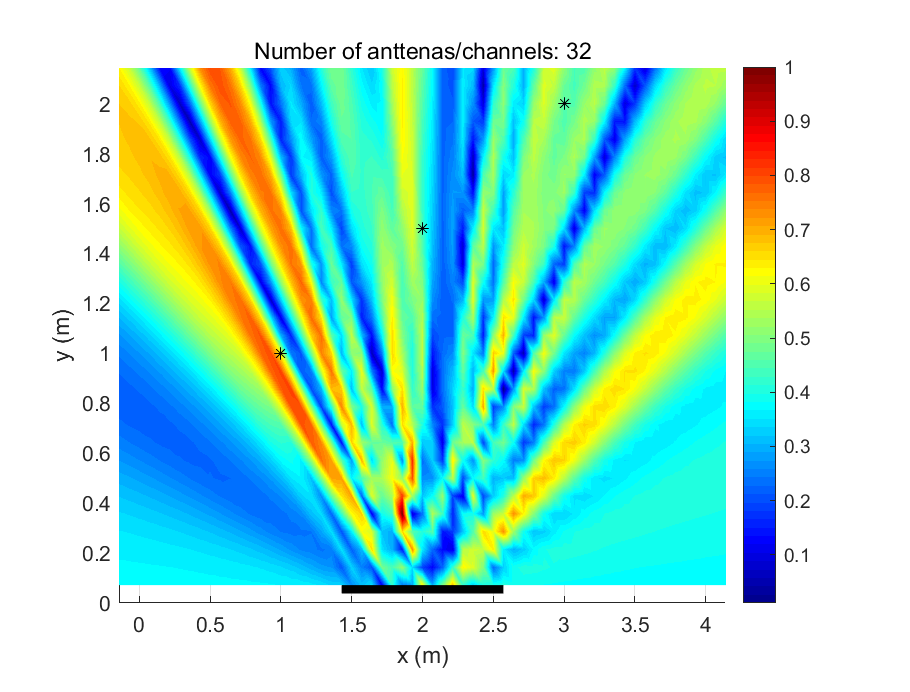
\includegraphics[width=1\textwidth]{figures/compare/CSI_freq1.eps}
    \caption{情形一频偏~直接成像}
  \end{subfigure}
  \begin{subfigure}[t]{.3\linewidth}
    \centering
    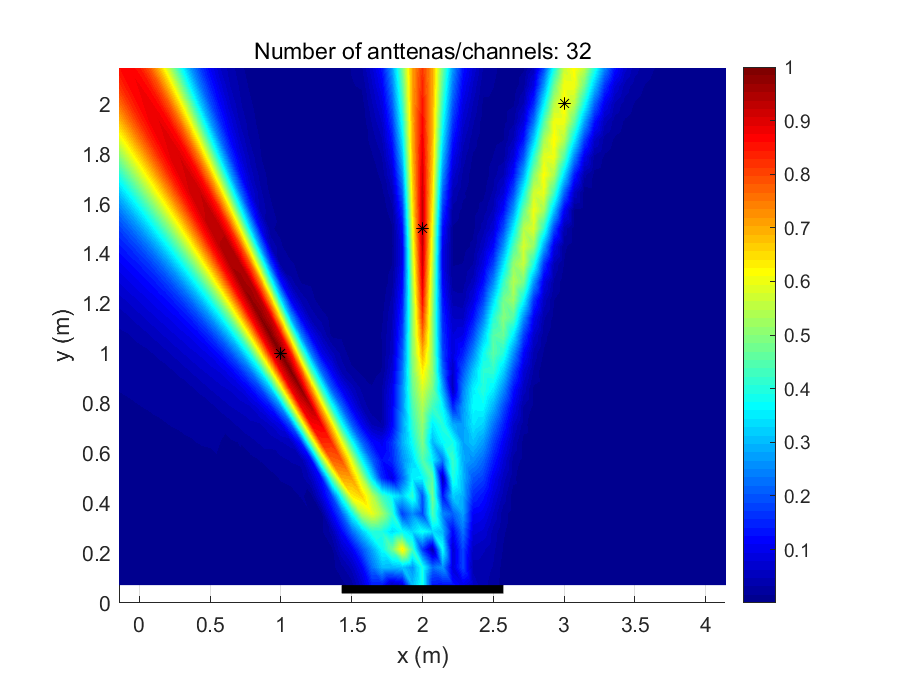
\includegraphics[width=1\textwidth]{figures/compare/CSI_freq2.eps}
    \caption{情形二频偏~直接成像}
  \end{subfigure}
  \\
  \begin{subfigure}[t]{.3\linewidth}
    \centering
    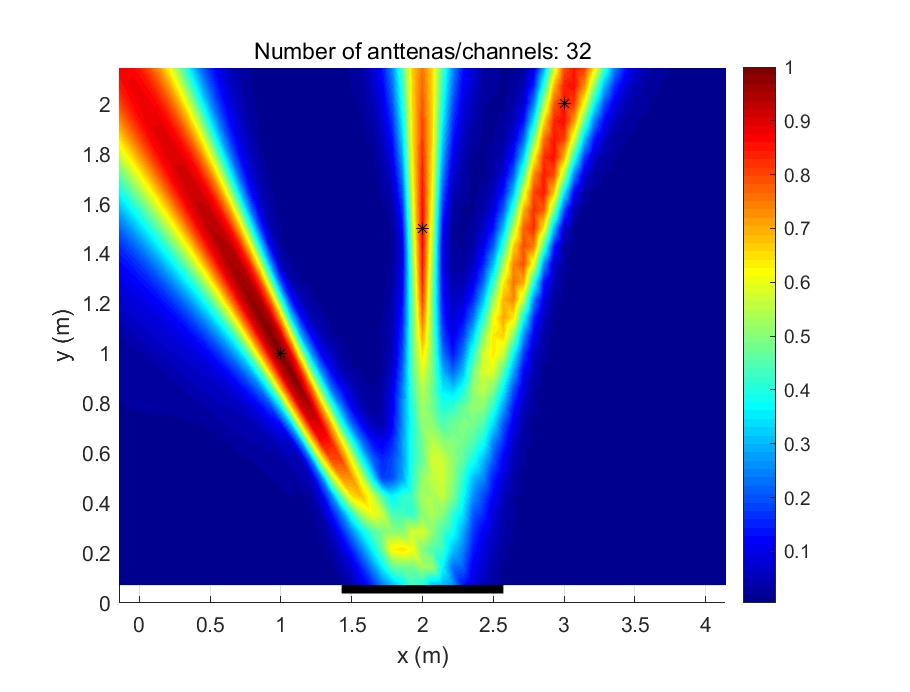
\includegraphics[width=1\textwidth]{figures/compare/TPF_without_freq.eps}
    \caption{未添加频偏~PARAFAC成像}
  \end{subfigure}
  \begin{subfigure}[t]{.3\linewidth}
    \centering
    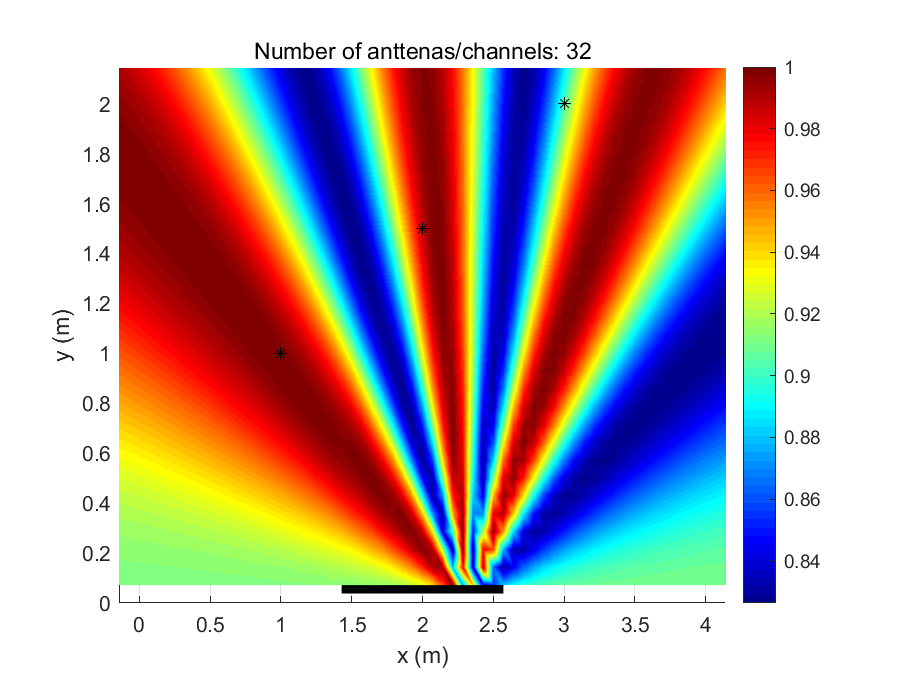
\includegraphics[width=1\textwidth]{figures/compare/TPF_freq1.eps}
    \caption{情形一频偏~PARAFAC成像}
  \end{subfigure}
  \begin{subfigure}[t]{.3\linewidth}
    \centering
    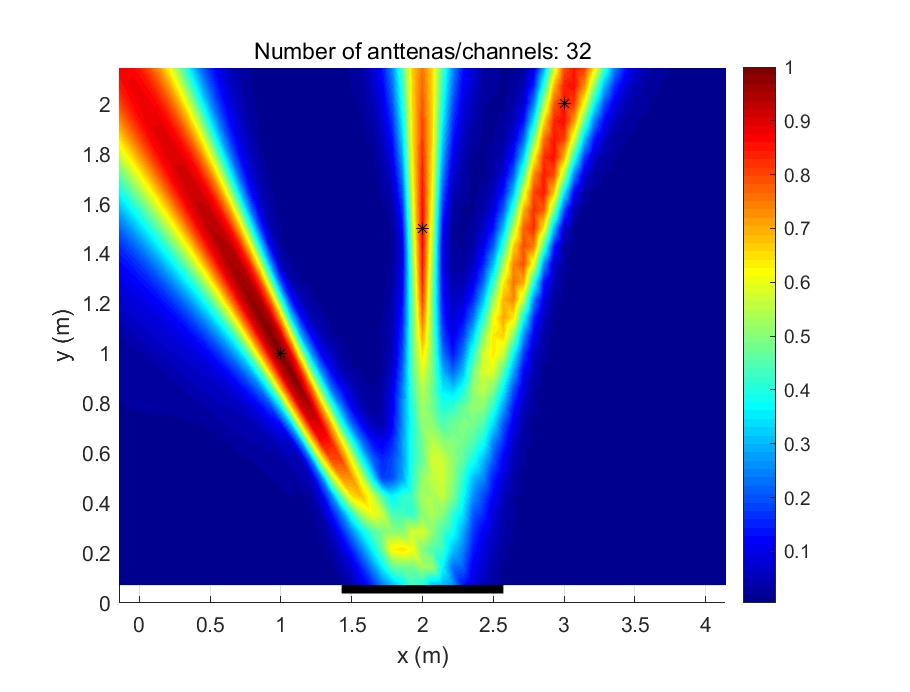
\includegraphics[width=1\textwidth]{figures/compare/TPF_freq2.eps}
    \caption{情形一频偏~PARAFAC成像}
  \end{subfigure}
  \\
  \begin{subfigure}[t]{.3\linewidth}
    \centering
    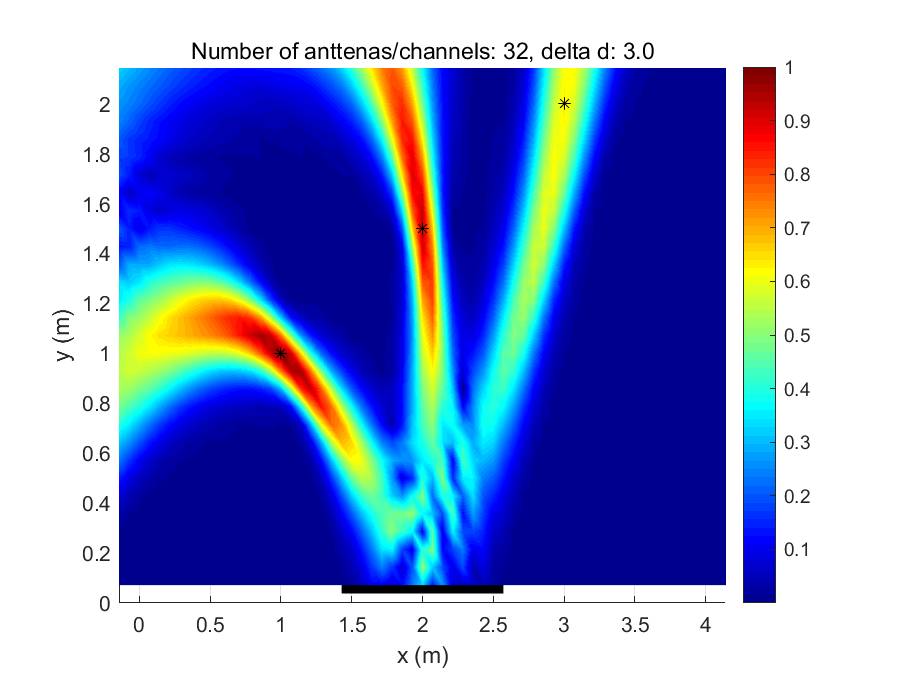
\includegraphics[width=1\textwidth]{figures/compare/CM_without_freq.eps}
    \caption{未添加频偏~共轭相乘成像}
  \end{subfigure}
  \begin{subfigure}[t]{.3\linewidth}
    \centering
    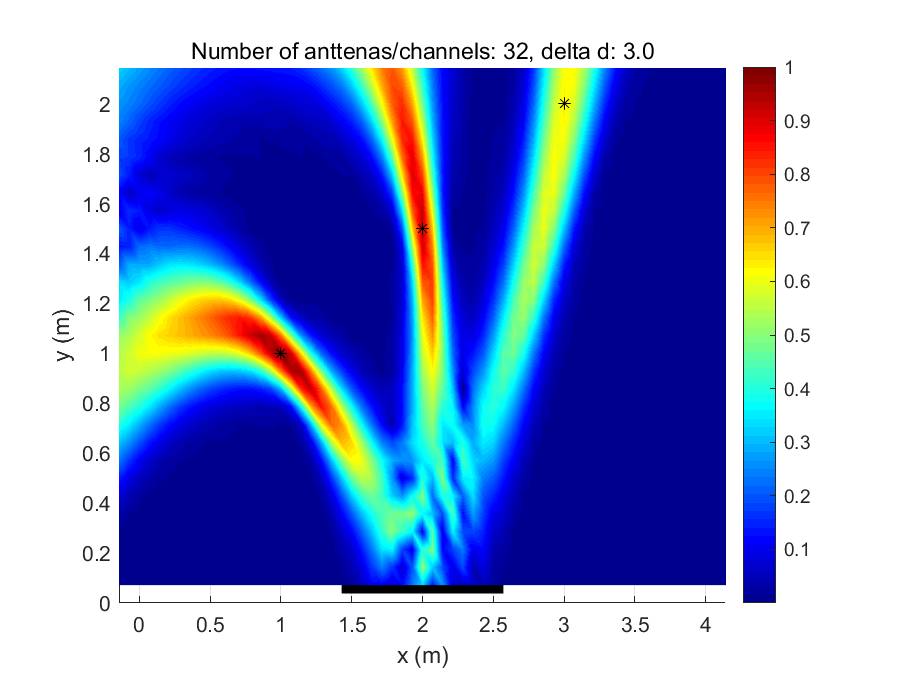
\includegraphics[width=1\textwidth]{figures/compare/CM_freq1.eps}
    \caption{情形一频偏~共轭相乘成像}
  \end{subfigure}
  \begin{subfigure}[t]{.3\linewidth}
    \centering
    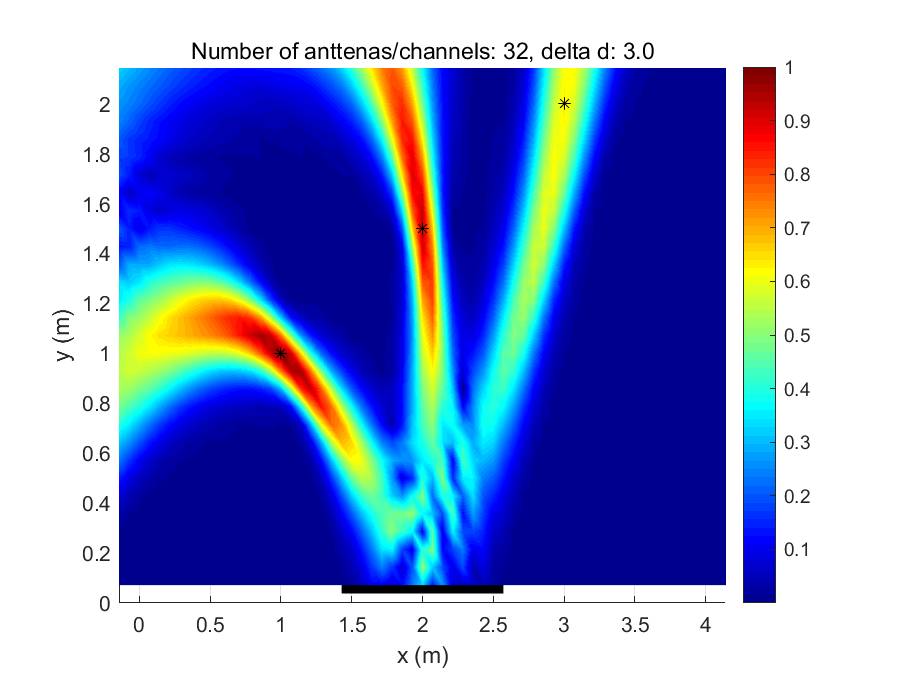
\includegraphics[width=1\textwidth]{figures/compare/CM_freq2.eps}
    \caption{情形二频偏~共轭相乘成像}
  \end{subfigure}
  \\
  \begin{subfigure}[t]{.3\linewidth}
    \centering
    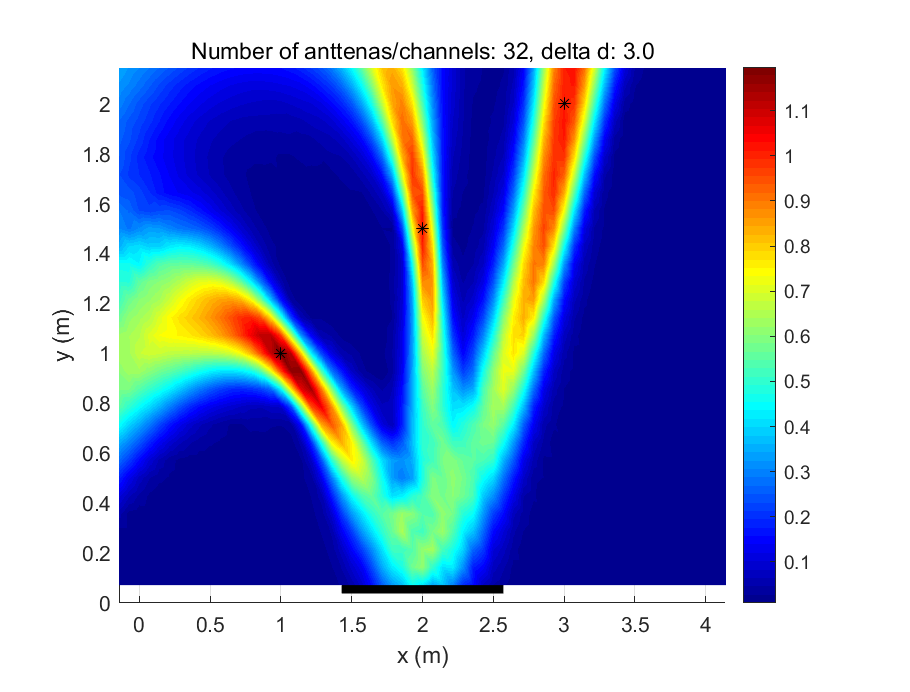
\includegraphics[width=1\textwidth]{figures/compare/TPF_CM_without_freq.eps}
    \caption{未添加频偏~结合PARAFAC与共轭相乘成像}
  \end{subfigure}
  \begin{subfigure}[t]{.3\linewidth}
    \centering
    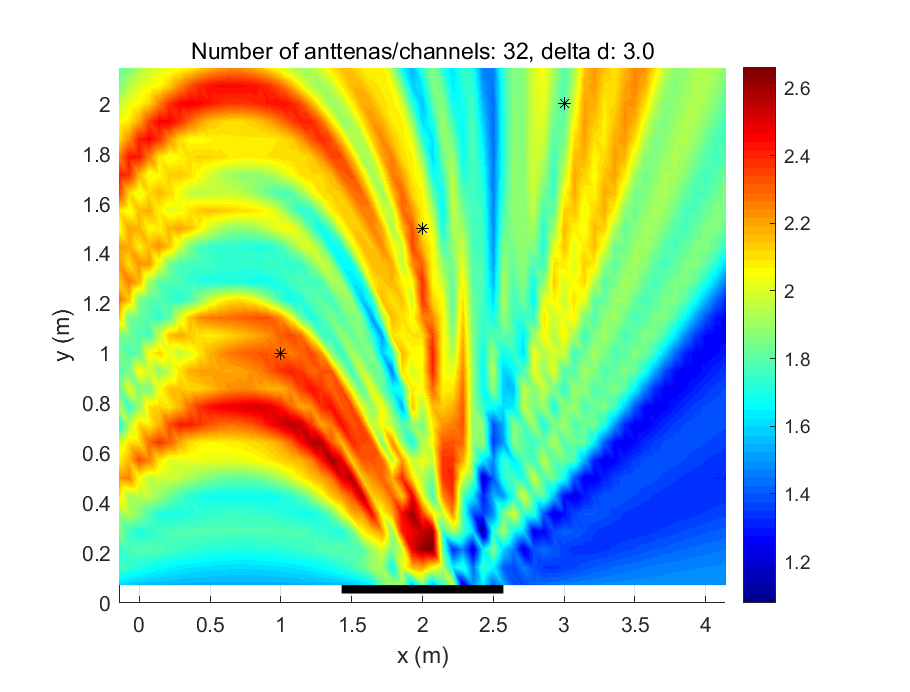
\includegraphics[width=1\textwidth]{figures/compare/TPF_CM_freq1.eps}
    \caption{情形一频偏~结合PARAFAC与共轭相乘成像}
  \end{subfigure}
  \begin{subfigure}[t]{.3\linewidth}
    \centering
    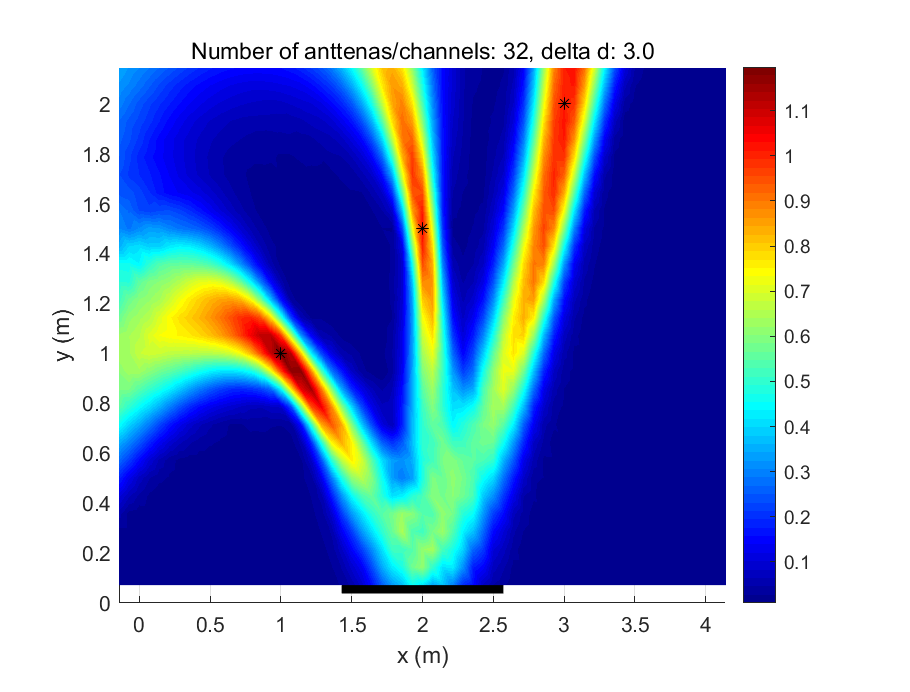
\includegraphics[width=1\textwidth]{figures/compare/TPF_CM_freq2.eps}
    \caption{情形二频偏~结合PARAFAC与共轭相乘成像}
  \end{subfigure}
  \caption{成像各种情况对比}\label{成像对比图}
\end{figure} 
  \section{应用前景:分布式成像}
\subsection{分布式成像仿真结果对比}
针对于前文的成像需要一个大的接收机阵列以及较大的两路接收机间距以消除频偏等问题,利用分布式
成像的方式是一个可能的潜在应用场景。这里给出了一个分布式成像的例子,如图~\ref{分布式成像仿真场景}所示。
需要注意的是,这里对$N=96$的接收阵列成像情形以及三个$N=32$的接收阵列分布式成像的结果进行了对比,并且
这里的成像结果考虑了对信源(发射机)的成像。
\begin{figure}[H]
  \centering
  \begin{subfigure}[t]{.45\linewidth}
    \centering
    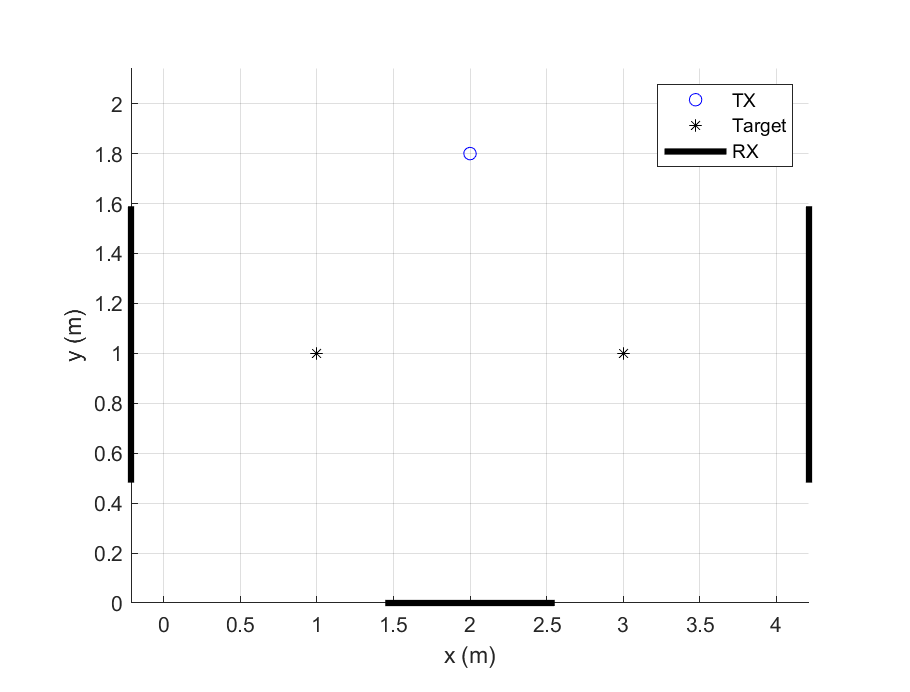
\includegraphics[width=1\textwidth]{figures/distribution/model1_circ.eps}
    \caption{$3$个$N=32$接收机阵列分布式成像}  
  \end{subfigure}
  \begin{subfigure}[t]{.45\linewidth}
    \centering
    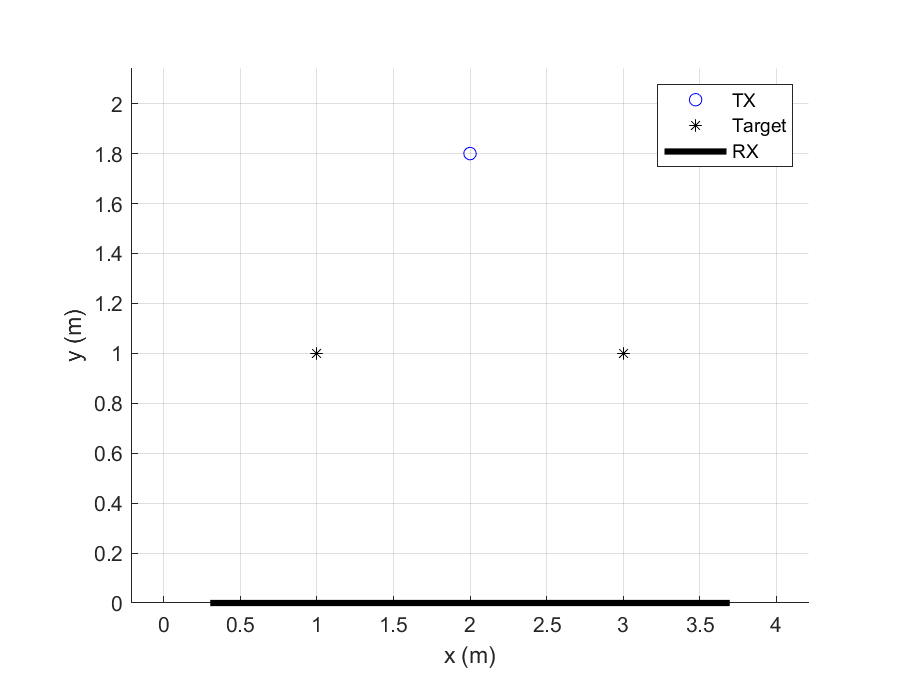
\includegraphics[width=1\textwidth]{figures/distribution/model1.eps}
    \caption{对比:单个$N=96$接收机阵列成像}
  \end{subfigure}
  \caption{分布式成像仿真场景}
  \label{分布式成像仿真场景}
\end{figure}
分布式成像添加的频偏与单阵列成像添加的频偏一致(服从公式~\eqref{情形二}),具体的仿真参数见表~\ref{分布式成像仿真设置},
仿真结果如图~\ref{分布式成像仿真结果}所示,可以看出,在理想成像或频偏影响较小的情况下,分布式成像具有和单阵列成像相近或更好的效果。
\begin{table}[htb]
  % h-here,t-top,b-bottom,优先级依次下降
      \begin{center}
      % 居中
          \caption{分布式成像仿真设置}\label{分布式成像仿真设置}
          \begin{tabular}{lc} % 三线表不能有竖线,l-left,c-center,r-right
              \toprule
              %三线表-top 线
              参数 & 值 \\
              \midrule
              %三线表-middle 线
              是否考虑对信源(发射机)成像 & 是(仿真多径设置了LOS径)\\
              是否考虑CSI频偏的影响 & 是\\
              考虑频偏的情形  & 服从公式~\eqref{情形二}\\
              采样频率偏移(SFO)   &   $\theta_{\text{sfo}}\sim N(0,100)$ Hz\\
              包检测误差(PDP)     &   $\theta_{\text{pdd}}\sim N(0,100)$ Hz\\
              载波频率偏移(CFO)   &   $\theta_{\text{cfo}}\sim N(0,1000)$ Hz\\
              成像目标数量(含信源)    & 3\\
              信源位置        &  $(2\text{米},1.8\text{米})$ \\
              成像目标的位置  & $(1\text{米},1\text{米})$,$(3\text{米},1\text{米})$ \\
              工作频点        & $4.2$GHz\\
              工作带宽      & 20MHz \\
              子载波数目      & 256\\
              发射机位置           & $(2\text{米},0\text{米})$\\
              接收机天线阵元数$N$      & $3*32$\\
              接收机天线阵元间隔    & 半波长(约$3.57$厘米)\\
              接收机位置           & 如图~\ref{分布式成像仿真场景}\\
              两路接收天线的位置差$\Delta_d$ & $1$米\\
              \bottomrule
              %三线表-底线
          \end{tabular}
      \end{center}
\end{table}

\begin{figure}[H]
  \centering
  \begin{subfigure}[t]{.3\linewidth}
    \centering
    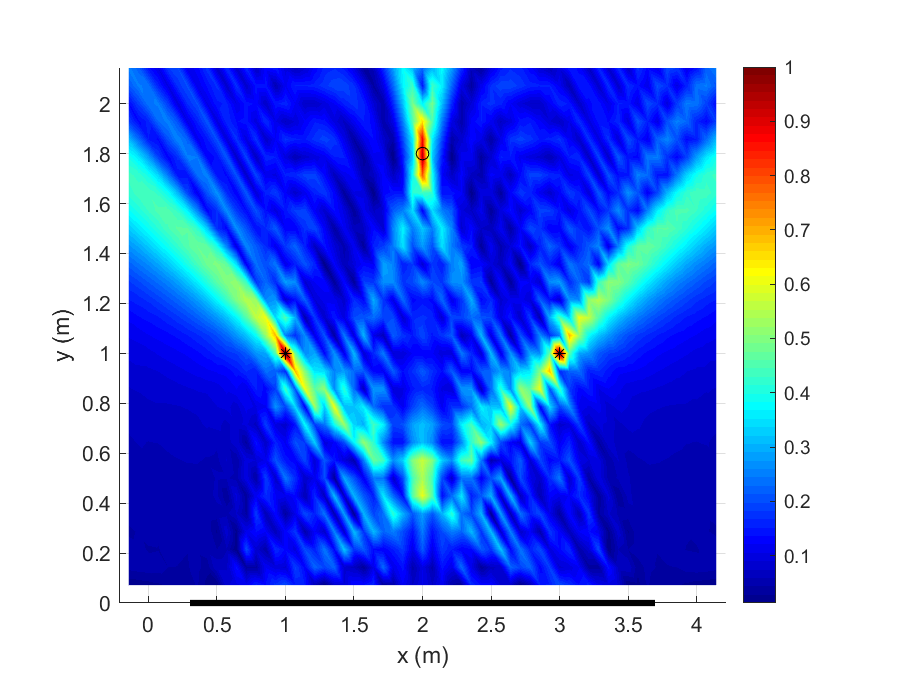
\includegraphics[width=1\textwidth]{figures/distribution/expected/array.eps}
    \caption{未添加频偏~单阵列成像}
  \end{subfigure}
  \begin{subfigure}[t]{.3\linewidth}
    \centering
    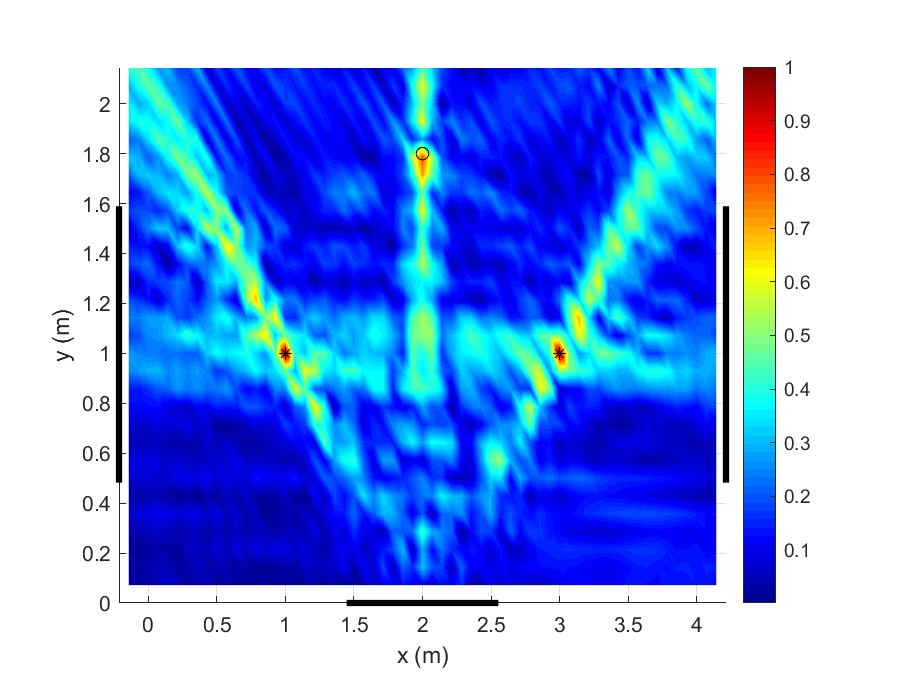
\includegraphics[width=1\textwidth]{figures/distribution/expected/joint.eps}
    \caption{未添加频偏~三个分布式阵列合并为单阵列}
  \end{subfigure}
  \begin{subfigure}[t]{.3\linewidth}
    \centering
    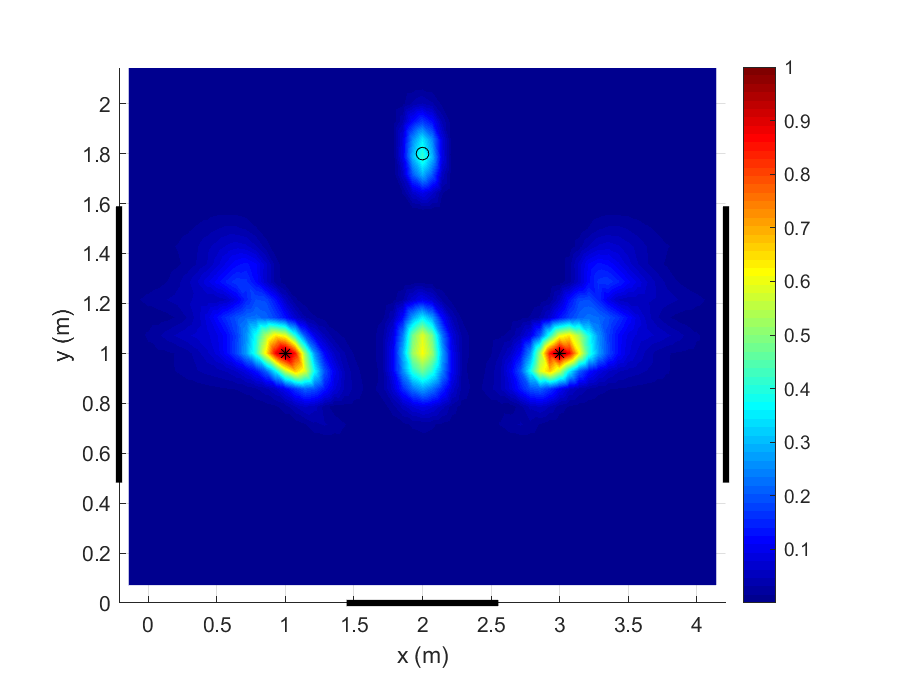
\includegraphics[width=1\textwidth]{figures/distribution/expected/multiplication.eps}
    \caption{未添加频偏~三个分布式阵列分别成像再相乘}
  \end{subfigure}
  \\
  \begin{subfigure}[t]{.3\linewidth}
    \centering
    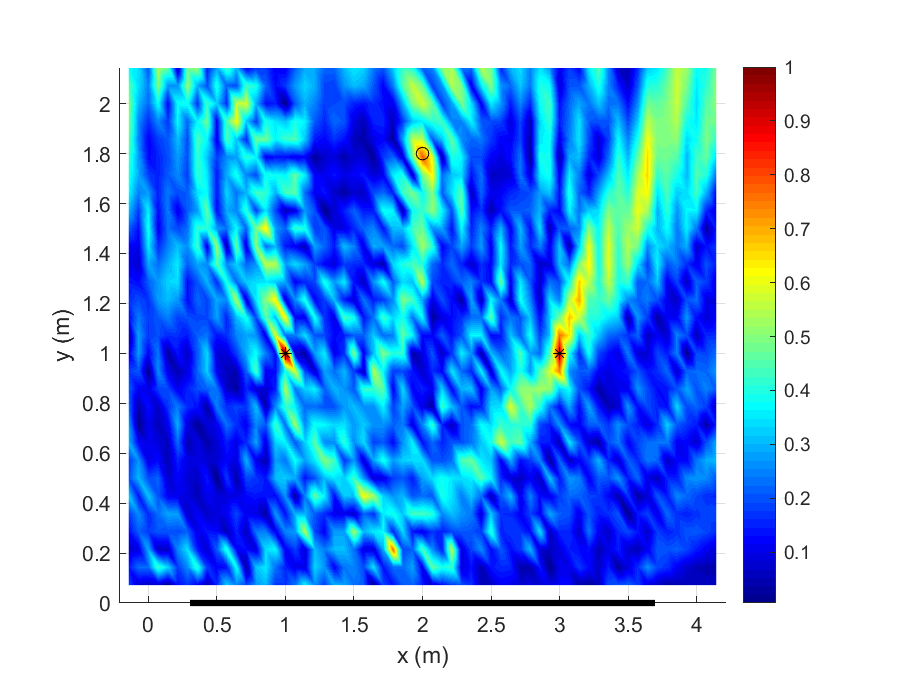
\includegraphics[width=1\textwidth]{figures/distribution/freq/array.eps}
    \caption{情形二频偏~单阵列成像}
  \end{subfigure}
  \begin{subfigure}[t]{.3\linewidth}
    \centering
    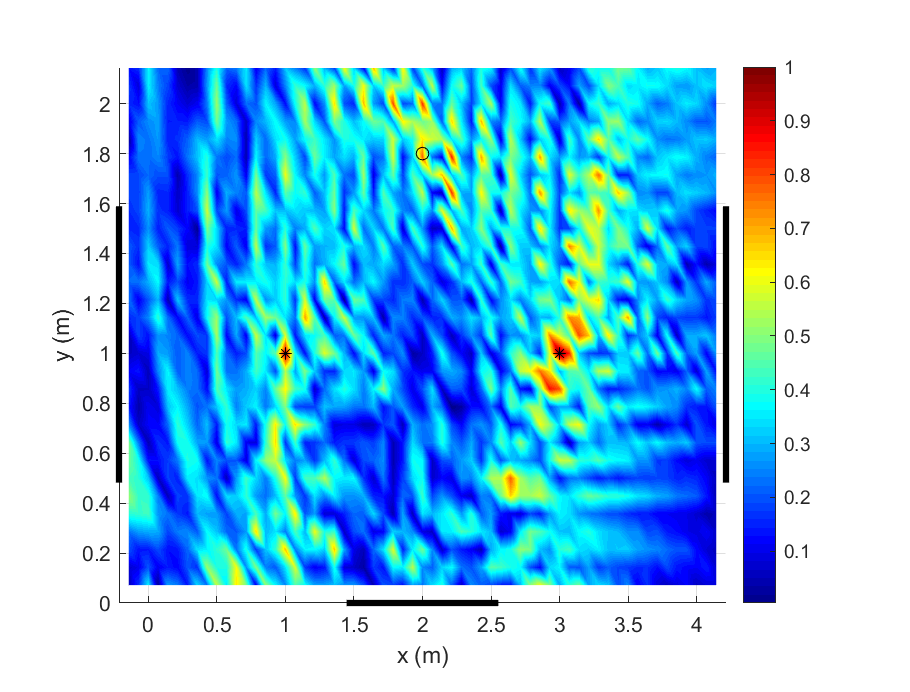
\includegraphics[width=1\textwidth]{figures/distribution/freq/joint.eps}
    \caption{情形二频偏~三个分布式阵列合并为单阵列}
  \end{subfigure}
  \begin{subfigure}[t]{.3\linewidth}
    \centering
    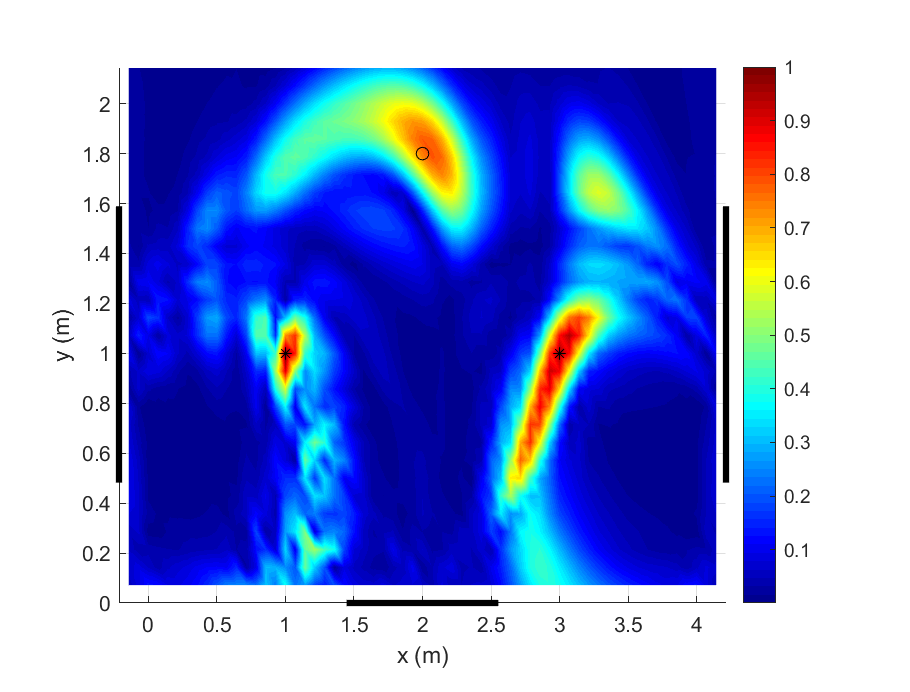
\includegraphics[width=1\textwidth]{figures/distribution/freq/multiplication.eps}
    \caption{情形二频偏~三个分布式阵列分别成像再相乘}
  \end{subfigure}
  \caption{分布式成像仿真结果}\label{分布式成像仿真结果}
\end{figure}

\begin{figure}[htb]
  \centering
  \begin{subfigure}[t]{.45\linewidth}
    \centering
    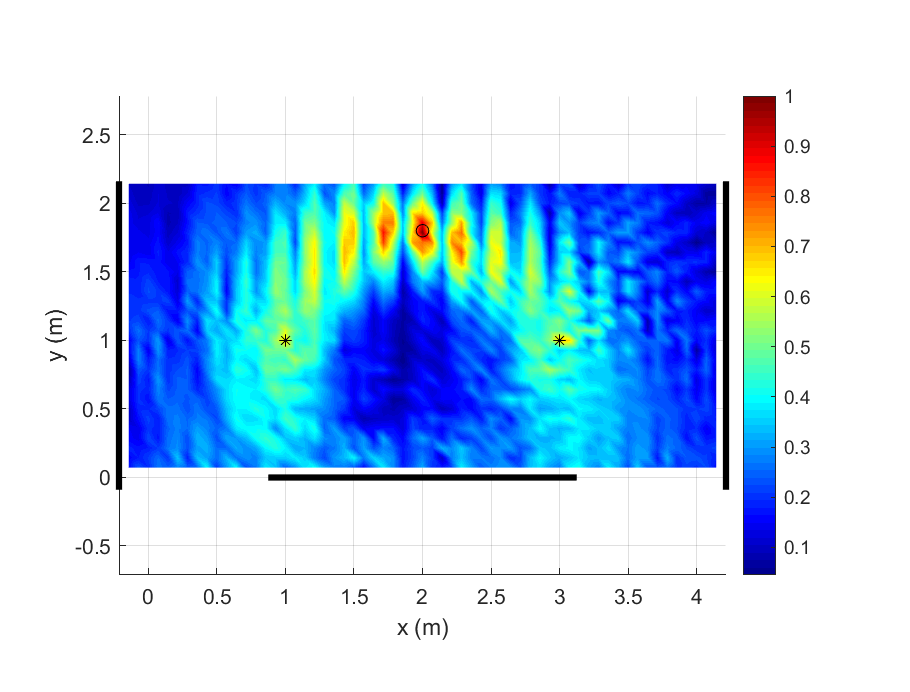
\includegraphics[width=\textwidth]{figures/distribution/TPF/1.eps}
    \caption{无频偏~每个子阵列分别加汉明窗}
  \end{subfigure}
  \begin{subfigure}[t]{.45\linewidth}
    \centering
    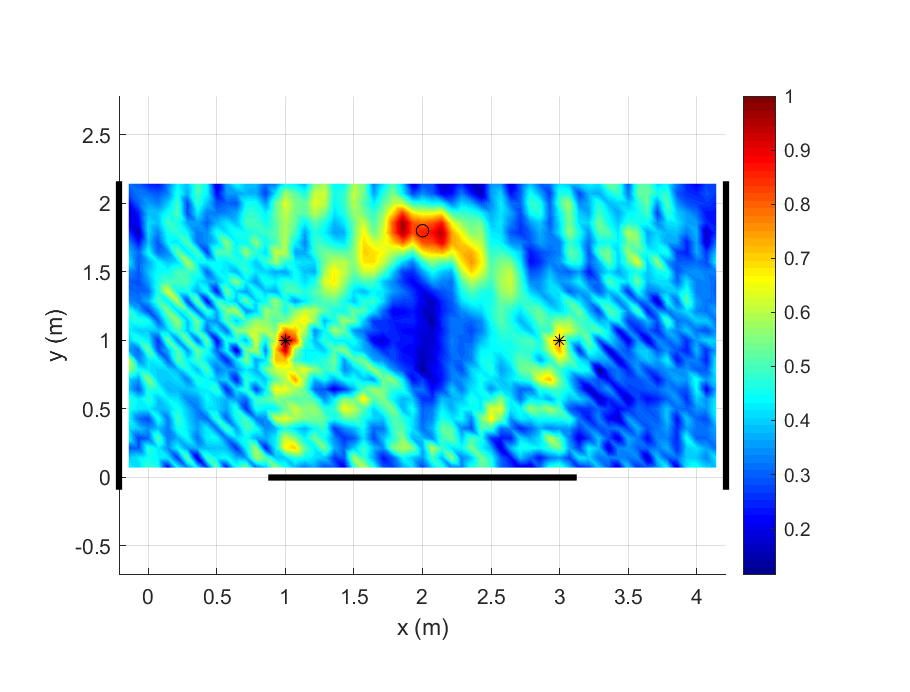
\includegraphics[width=\textwidth]{figures/distribution/TPF/2.eps}
    \caption{情形二频偏~每个子阵列分别加汉明窗}
  \end{subfigure}
  \begin{subfigure}[t]{.45\linewidth}
    \centering
    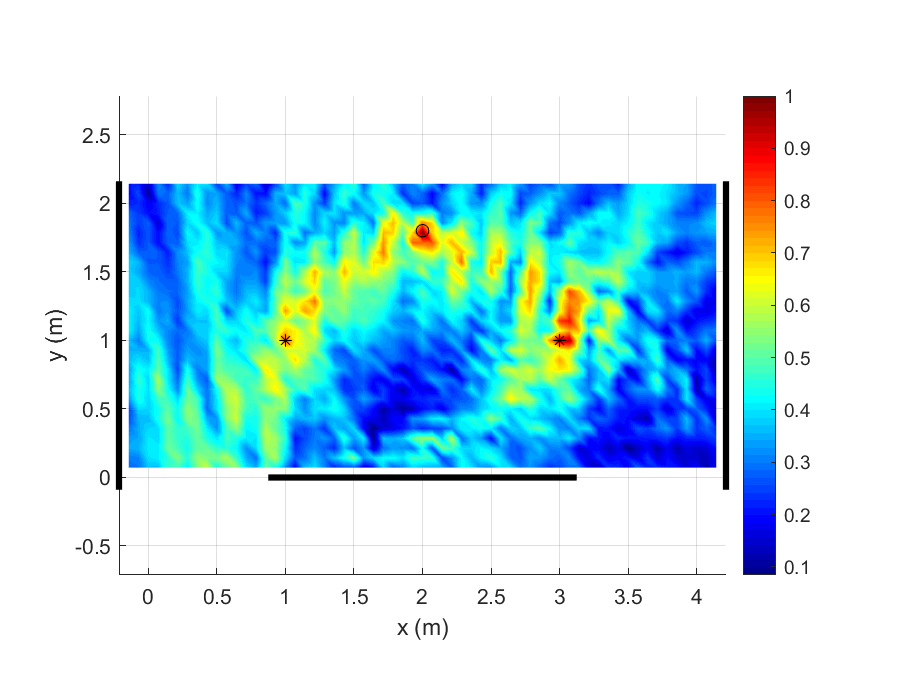
\includegraphics[width=\textwidth]{figures/distribution/TPF/3.eps}
    \caption{无频偏~子阵列串联后整体加窗}
  \end{subfigure}
  \begin{subfigure}[t]{.45\linewidth}
    \centering
    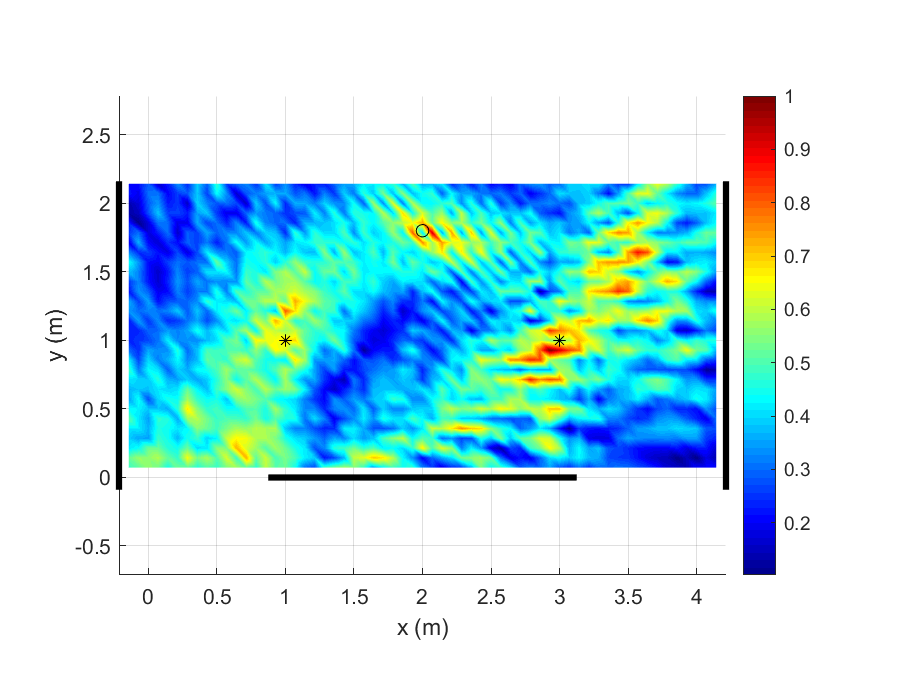
\includegraphics[width=\textwidth]{figures/distribution/TPF/4.eps}
    \caption{情形二频偏~子阵列串联后整体加窗}
  \end{subfigure}
  \caption{结合PARAFAC算法的分布式成像仿真结果}
  \label{TPF分布式}
\end{figure}

\subsection{结合PARAFAC算法的分布式成像仿真结果}
结合PARAFAC算法与共轭相乘消除频偏的仿真采取$N=3*64$,$\delta_d=0.8$米的接收天线阵列,其余参数与表~\ref{分布式成像仿真设置}一致。
仿真结果如图~\ref{TPF分布式}所示,需要注意的是,这里我们还尝试了子阵列成像结果分别汉明窗以及子阵列联合成像结果加统一的汉明窗对结果的影响,
可以看出,子阵列分别加汉明窗具有更好的成像效果。 
  \section{基于数控导轨的简单实测成像}
\subsection{实验设置}
本文基于AD9361软件无线电开发板,以及数控滑轨实现了一个简单的基于CSI的成像系统。
\begin{itemize}
  \item 利用MATLAB中的WLAN toolbox\cite{wlantoolbox}产生一段IEEE 802.11ax\cite{ong2011ieee}中的"空数据包"(NDP: Null Data Packet)波形\cite{perahia2013next},再经过AD9361平台发送和接收信号。
  \item 通过数控滑轨搭载接收天线移动,模拟一个巨大的接收天线阵列。(需要注意的是,为了便于自动化的测试,本实验实现了对福誉科技数控轨道\cite{fuyu}的简单MATLAB驱动。)
  \item (Channel Sounding)通过WLAN toolbox对接收基带信号处理(移除循环前缀、粗/细频偏估计等),再通过发射机发送的NDP信号中的长训练序列(L-LTF: Legacy-Long Training Field)信号做信道估计,进而得到CSI\cite{ma2019wifi}\cite{perahia2013next}。
\end{itemize}
后续实验设置与仿真设置类似,Wi-Fi信号工作中心频点为$4.2$GHz,带宽为$20$MHz,并考虑了是/否对LOS径(信源)的成像。
\subsection{部分实测场景及实测结果}
\subsubsection{实验场景一:$N=32$对目标/信源成像}
图~\ref{32实验场景},图~\ref{32结果}分别展示了利用数控轨道模拟的含32个阵元的接收机阵列对单个目标,单个信源的成像场景及结果。
可以看出,本成像方案可以有效的对目标和信源成像。
\begin{figure}[H]
  \centering
  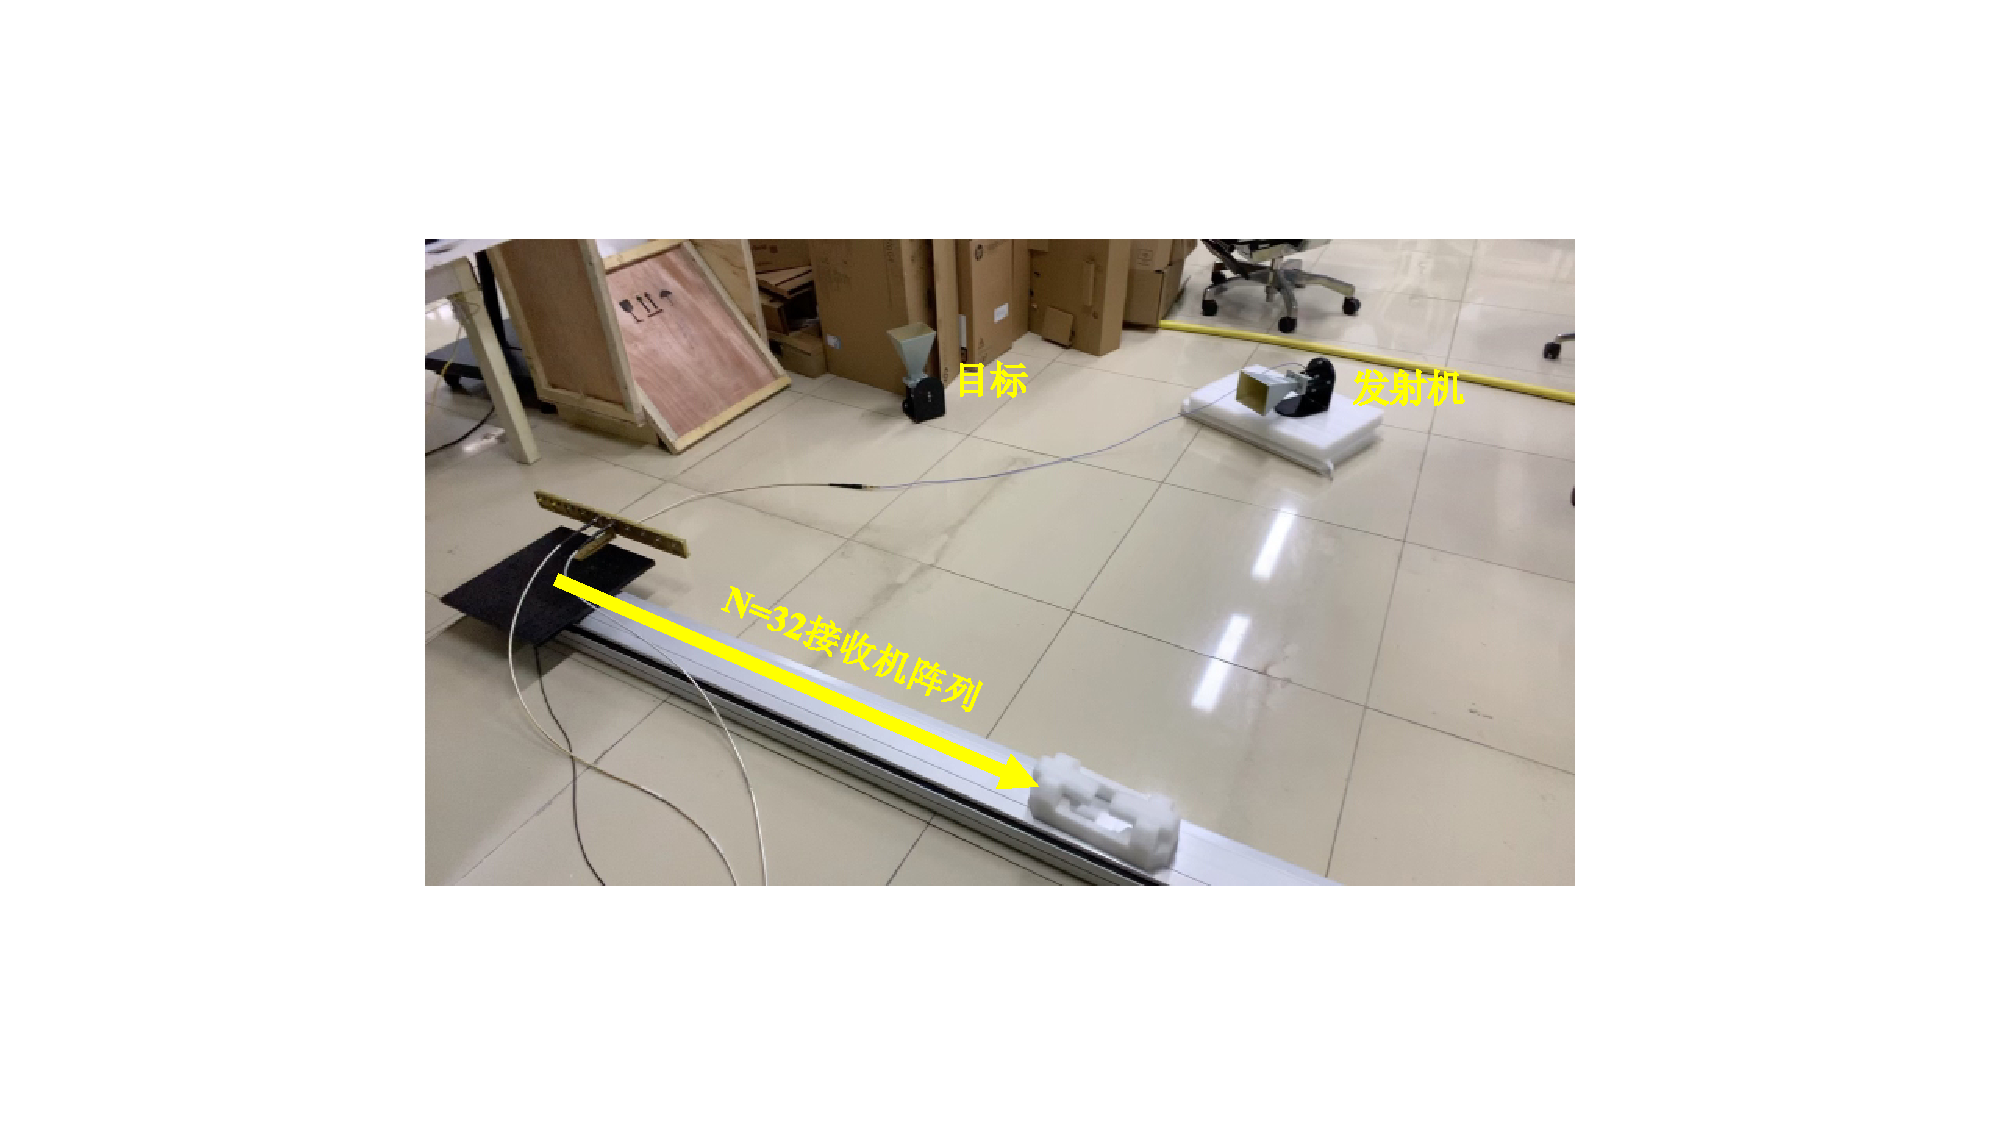
\includegraphics[width=.8\textwidth]{figures/exp/32.pdf}
  \caption{$N=32$实验场景}
  \label{32实验场景}
\end{figure}
\begin{figure}[H]
  \centering
  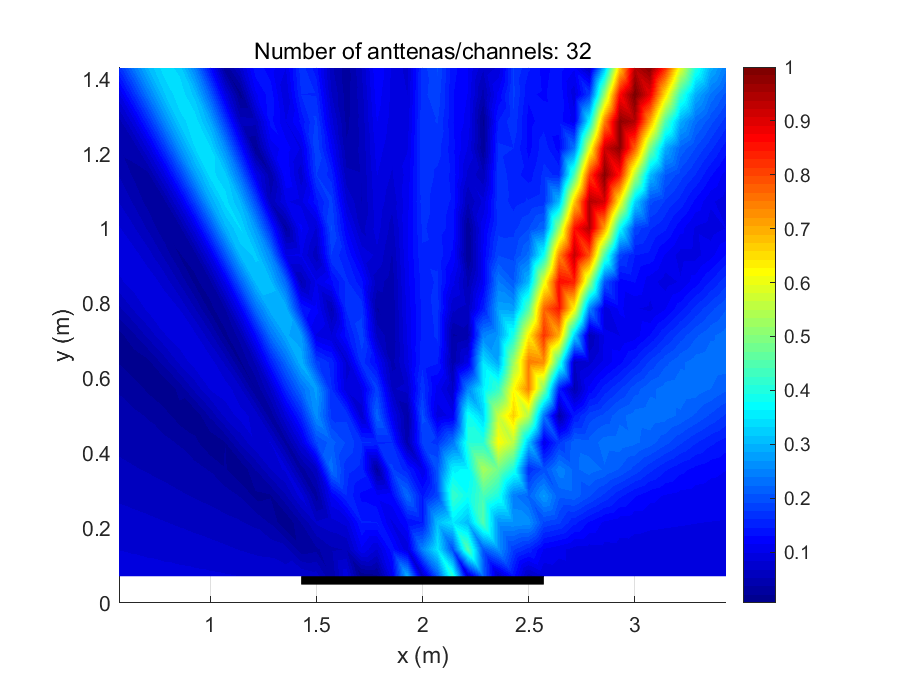
\includegraphics[width=.8\textwidth]{figures/exp/N32.eps}
  \caption{$N=32$对目标/信源成像结果}
  \label{32结果}
\end{figure}
\subsubsection{实验场景二:$N=64$对目标成像}
本小节对另一种成像场景进行了实测:不考虑对LOS径(信源)成像,而仅仅对目标成像。图~\ref{左},图~\ref{左结果}分别展示了利用数控轨道模拟的含64个阵元的接收机阵列对单个位于阵列左侧目标的成像场景及结果。
而图~\ref{右},图~\ref{右结果}分别展示了利用数控轨道模拟的含64个阵元的接收机阵列对单个位于阵列右侧目标的成像场景及结果。可以看出,在该场景下,本成像方案同样具有不错的效果。
\begin{figure}[H]
  \centering
  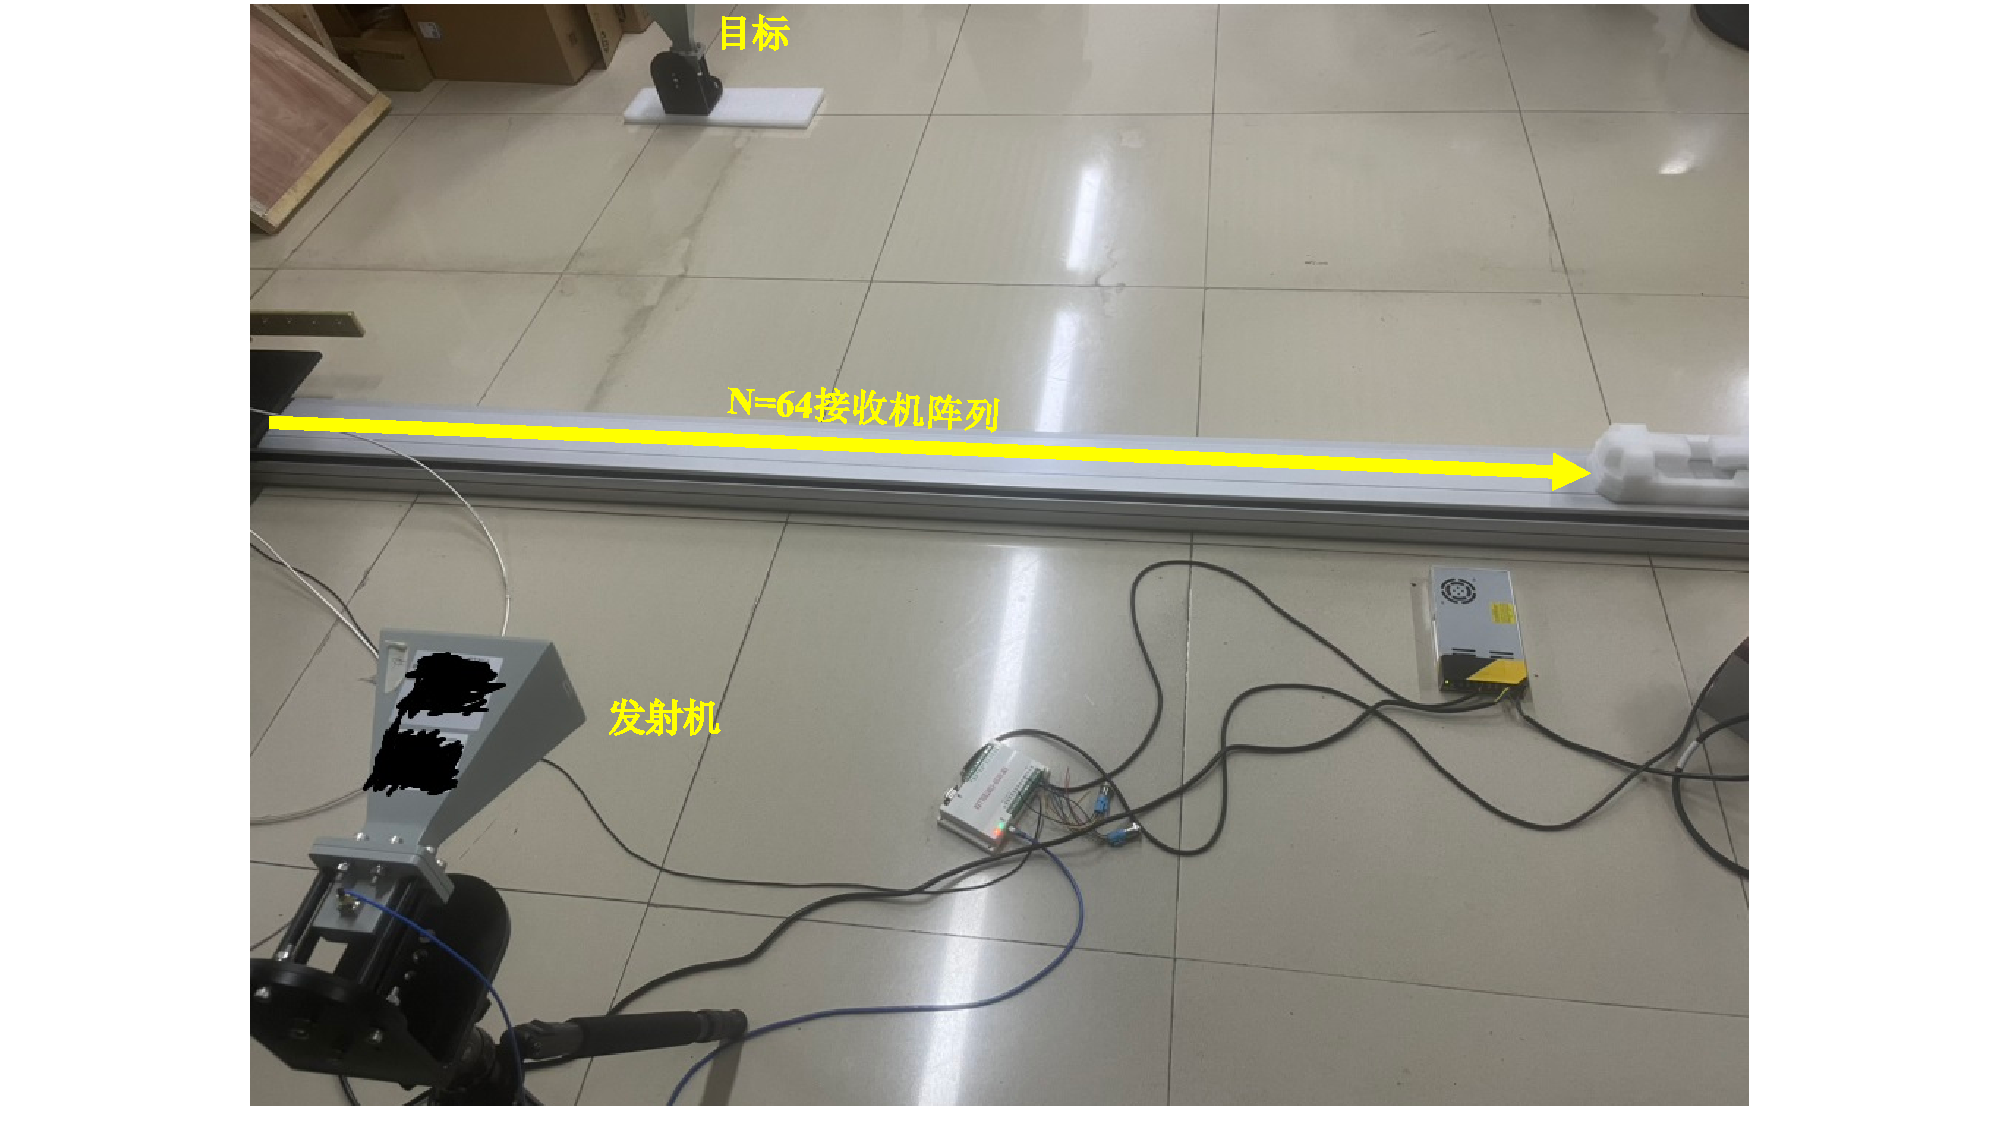
\includegraphics[width=.8\textwidth]{figures/exp/left.pdf}
  \caption{$N=64$对单目标成像场景(目标位于阵列左侧)}
  \label{左}
\end{figure}
\begin{figure}[H]
  \centering
  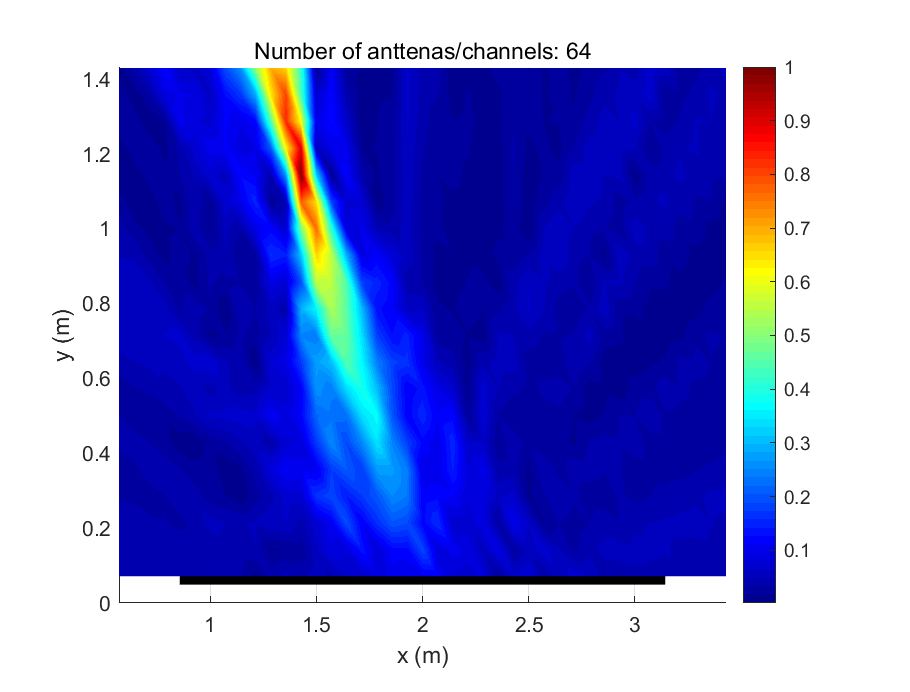
\includegraphics[width=.8\textwidth]{figures/exp/N64_left.eps}
  \caption{$N=64$对单目标成像结果(目标位于阵列左侧)}
  \label{左结果}
\end{figure}
\begin{figure}[H]
  \centering
  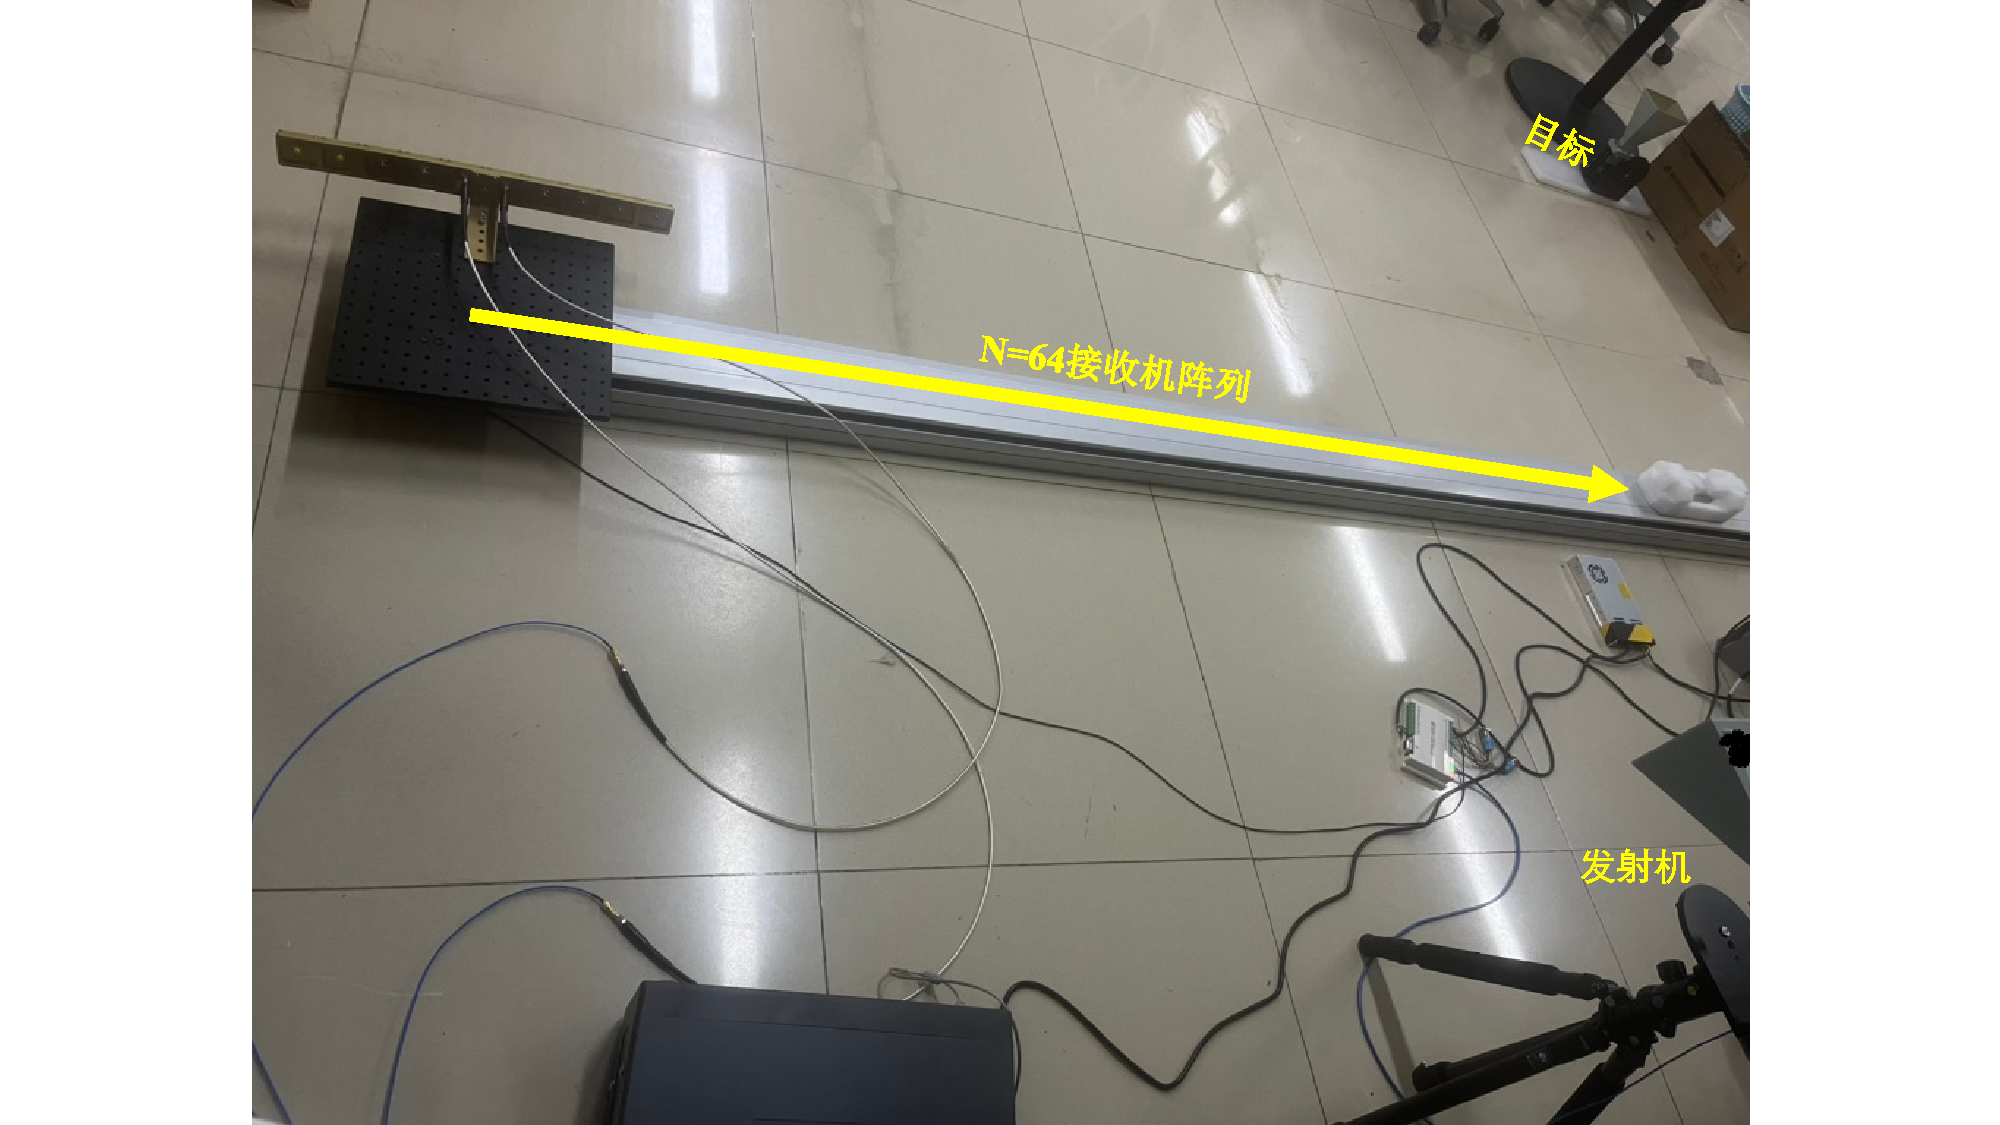
\includegraphics[width=.8\textwidth]{figures/exp/right.pdf}
  \caption{$N=64$对单目标成像场景(目标位于阵列右侧)}
  \label{右}
\end{figure}
\begin{figure}[H]
  \centering
  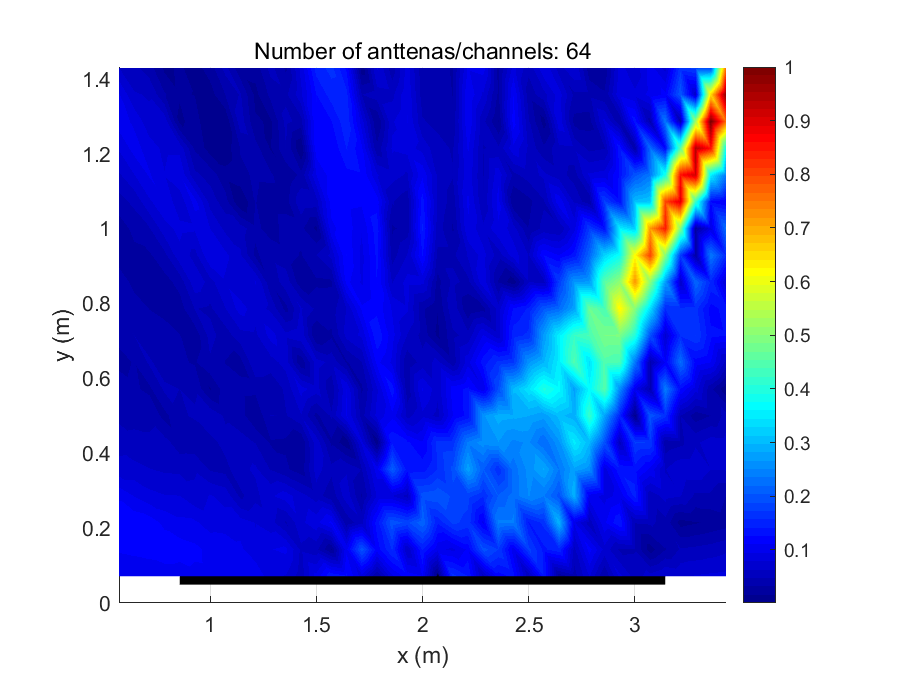
\includegraphics[width=.8\textwidth]{figures/exp/N64_right.eps}
  \caption{$N=64$对单目标成像场景(目标位于阵列右侧)}
  \label{右结果}
\end{figure} 
  \section{总结}
仿真与实测表明,基于Wi-Fi的室内近场成像可以有效地实现对室内信源,反射物的探测、定位与成像。 
\end{spacing}
% % !Mode:: "TeX:UTF-8"
% !TEX program  = xelatex
\section{免责声明}
\begin{enumerate}[label={\alph*)}]
    \item 本模板的发布遵守 \LaTeX\ Project Public License,使用前请认真阅读协议内容。
    \item 南方科技大学教学工作部只提供毕业论文写作指南,不提供官方模板,也不会授权第三方模板为官方模板,所以此模板仅为写作指南的参考实现,不保证格式审查老师不提意见. 任何由于使用本模板而引起的论文格式审查问题均与本模板作者无关。
    \item 任何个人或组织以本模板为基础进行修改,扩展而生成的新的专用模板,请严格遵守 \LaTeX\ Project Public License 协议。由于违犯协议而引起的任何纠纷争端均与本模板作者无关。
\end{enumerate}

% % !Mode:: "TeX:UTF-8"
% !TEX program  = xelatex
\section{文类接口}
文类的接口的命名均为汉字,意思为字面意思,如有疑问,欢迎在 GitHub 提出 \href{https://github.com/Iydon/sustechthesis/issues}{Issues}。

\subsection{汉化字号接口}
本接口主要使用 \texttt{ctex} 宏包。

\verbbox{\初号},\verbbox{\小初},\verbbox{\一号},\verbbox{\小一},\verbbox{\二号},\verbbox{\小二},\verbbox{\三号},\verbbox{\小三},\verbbox{\四号},\verbbox{\小四},\verbbox{\五号},\verbbox{\小五},\verbbox{\六号},\verbbox{\小六},\verbbox{\七号},\verbbox{\八号}。


\subsection{汉化字体接口}
可能本机上部分字体不存在,导致部分字体无法使用。

\verbbox{\宋体},\verbbox{\黑体},\verbbox{\仿宋},\verbbox{\楷书},\verbbox{\隶书},\verbbox{\幼圆},\verbbox{\雅黑},\verbbox{\苹方}。


\subsection{字体效果接口}

建议在正文时使用 \verb|\textbf{}|,\verb|\textit{}| 调用\textbf{粗体}与\textit{斜体}。

It is recommended to use \verb|\textbf{}|,\verb|\textit{}| to call \textbf{Bold} and \textit{ItalicFont}.

\verbbox{\粗体},\verbbox{\斜体}。


\subsection{格式相关接口}
\subsubsection{命令}
例子请参考前文,在写论文初期,可以注释掉标题页等不必要信息,以加快编译速度。

\verbbox{\设置信息},\verbbox{\目录},\verbbox{\下划线},\verbbox{\中文标题页},\verbbox{\英文标题页},\verbbox{\中文诚信承诺书},\verbbox{\英文诚信承诺书},\verbbox{\摘要标题},\verbbox{\参考文献},\verbbox{\附录},\verbbox{\致谢}。

\subsubsection{环境}
摘要环境均需一个参数,为关键词:\verb|\begin{}{}...\end{}|。

\verbbox{中文摘要},\verbbox{英文摘要}。

% % !Mode:: "TeX:UTF-8"
% !TEX program  = xelatex

\section{一些样例}

\subsection{表格}

\begin{table}[htb]
% h-here,t-top,b-bottom,优先级依次下降
    \begin{center}
    % 居中
        \caption{表格的标题应该放在上方}\label{table}
        \begin{tabular}{lc} % 三线表不能有竖线,l-left,c-center,r-right
            \toprule
            %三线表-top 线
            Example & Result \\
            \midrule
            %三线表-middle 线
            Example1          & 0.25 \\
            Example2          & 0.36 \\
            \bottomrule
            %三线表-底线
        \end{tabular}
    \end{center}
\end{table}

\subsection{参考文献}

参考文献如是\cite{Nicholas1998Handbook}。

% \begin{figure}[htb]
    \centering
    \includegraphics[width=.5\textwidth]{example-image-a}
    \caption{自带测试图片---Test image}\label{F:test-a}
    % 图片的标题应该在下方
\end{figure}

\begin{figure}[htb]
    \centering
    \begin{subfigure}[t]{.3\linewidth}
        \centering
        \includegraphics[width=1\textwidth]{example-image-a}
        \caption{子图-自带测试图片---Test image}\label{F:test-b-sub-a}
    \end{subfigure}
    \begin{subfigure}[t]{.3\linewidth}
        \centering
        \includegraphics[width=1\textwidth]{example-image-a}
        \caption{子图-自带测试图片---Test image}\label{F:test-b-sub-b}
    \end{subfigure}
    \begin{subfigure}[t]{.3\linewidth}
        \centering
        \includegraphics[width=1\textwidth]{example-image-a}
        \caption{子图-自带测试图片---Test image}\label{F:test-b-sub-b}
    \end{subfigure}
    \caption{自带测试图片---Test image}\label{F:test-b}
\end{figure}
% % !Mode:: "TeX:UTF-8"
% !TEX program  = xelatex
\section{\LaTeX\ 入门}
请参考 \href{https://tex.readthedocs.io/zh_CN/latest/}{在线文档},包括学习资源及学习路径。欢迎在 GitHub 上提出 \href{https://github.com/Iydon/tex/issues}{Issues}。
\clearpage
\clearpage
\参考文献
  \printbibliography[heading=none]\clearpage
% \附录
%   % !Mode:: "TeX:UTF-8"
% !TEX program  = xelatex
\section*{数据获取函数}\label{A:data}
\Python{utils.py}{code/examples/utils.py}
\clearpage
\致谢
  本项工作是我在华为技术有限公司无线技术实验室实习时完成,感谢我的学术导师王锐以及公司的同事韩霄、杜瑞对我的指导。
当然,也要感谢我的实习生学长谢海亮对我仿真,实验工作无微不至的指引和帮助。
\end{document}
